\chapter{Micro-Doppler Analysis}
This chapter gives a general discussion of micro-Doppler analysis, which is mandatory to understand how it is possible to classify a drone target by knowing only its radar backscattered signal. In particular, for a specialized drone detection radar, being able to distinguish a drone from another object is crucial. It's possible to understand by the previous chapter that one of the most used techniques to discriminate a drone from any other object is the micro-Doppler analysis.
This is possible by analyzing the temporal variation of the frequency of the signal received by a drone. As we will see now, these frequency variations are characteristic of drones because these have characteristic pattern. In fact, in this case we talk about 'signature' of a drone on the time-frequency plane. This characteristic frequency variation is due to the presence of rotating blades which add an additional Doppler contribution to that due to the object's translation velocity. This chapter analyses the signal characteristics in the time-frequency domain and the models that can be adopted to describe the signal received by a rotor blades. The differences between the two models considered are highlighted with the possibility to represent the micro-Doppler effect also on the Range-Time plane under specific conditions. Then, it is given a discussion on the effect of cell migration and on the possible ways of dealing with it. In the end the possible ways to conduct the micro-Doppler analysis for the different radar technologies are summarized.
%aggiungere ultima parte del capitolo: Modelli approssimati, cell migration e range slow time plane.     In this case the possible complications due to the cell migration effect are described. Ways of dealing with this effect are then highlighted. 

\section{Doppler effect in radar}
The Doppler effect, discovered in 1842 by Christian Doppler, has been used in radar since the 1950s for target recognition, speed measurement, identifying moving targets and imaging. The Doppler effect occurs when a target moves at a relative speed to the radar, so the signal it reflects will have a different frequency to the signal transmitted by the radar.
Assuming the radar transmits a signal $s(t)$ at the reference frequency $f_{0}$ with amplitude $u(t)$ and phase $\Phi = 2\pi f_{0} t$:

\begin{equation}
s(t)=u(t) \exp \left(j 2\pi f_{0} t\right)
\end{equation}

Supposing there is a target at distance $R_{0}$ approaching the radar with radial velocity with respect to it $v_{r}$, so the range equation for that target is:

\begin{equation}
R\left(t\right)=R_{0}-v_{r} t
\label{rangeradar}
\end{equation}

The signal backscattered by the target and received by the radar will have the following form:

\begin{equation}
s_{r}(t) =\sigma u\left(t-t_{d}\right) \exp \left(j 2\pi f_{0}\left(t-t_{d}\right)\right)
\label{reflectedsignal}
\end{equation}

Where $\sigma$ is the RCS contributions of target and $t_{d}$ is the two way delay from radar to target that is expressed as follow:

\begin{equation}
t_{d}=\frac{2 R\left(t\right)}{c}
\label{2waydelay}
\end{equation}

By inserting the \ref{2waydelay} in \ref{rangeradar}:

\begin{equation}
t_{d}=\frac{2\left(R_{0}-v_{r} t\right)}{c-v_{r}}
\label{delayfinal}
\end{equation}

Inserting \ref{delayfinal} in \ref{reflectedsignal}:

\begin{equation}
s_{r}(t)=\sigma u\left(\frac{c+v_{r}}{c-v_{r}} t-\frac{2 R_{0}}{c-v_{r}}\right) \exp \left[j 2\pi f_{0}\left(\frac{c+v_{r}}{c-v_{r}} t-\frac{2 R_{0}}{c-v_{r}}\right)\right]
\label{reflectedsigfinal}
\end{equation}

Making the subtraction between frequency of received signal from target and original frequency of transmitted signal and considering the velocity of the light much greater than the speed of the target:
\begin{equation}
\frac{c+v_{r}}{c-v_{r}} (2\pi f_{0})-(2\pi f_{0})=\frac{2 v_{r}}{c-v_{r}} (2\pi f_{0}) \approx \frac{2 v_{r}}{c} (2\pi f_{0})=2 \pi \frac{2 v_{r}}{\lambda}
\end{equation}

At the end the frequency shift found in the reflected signal due to the Doppler effect is therefore:

\begin{equation}
f_{\mathrm{d}}=\frac{2 v_{r}}{\lambda}
\end{equation}


\section{Scattering center model}
%inseriire il modello di scatters point che costituiscono un target considerando anche il contributo di fase, dicendo che utilizzando la X band a 9GHz e avendo una lunghezza d'onda di 3 centrimeti sono sufficienti per utilizzare il modello nel caso di droni le cui dimensioni sono nell'ordine di decine di centimetri?
The phenomenon of basckscattering that occurs in radars is generally complex and depends on several factors such as wavelength, polarisation, target rcs etc. A widely used model that greatly simplifies the modelling of this phenomenon is the scattering center model. When dimensions of target are large enough than the used wavelength is possible to consider the target as a composition of more scatter points. Each one give its amplitude and phase contribution. The base assumption to make correct this model is to consider the first law of electromagnetic scattering theory, so the approximation of Maxwell equation in high frequency and the assumption that the target size is larger than the wavelength. In the case of X band frequencies, the wavelength is in the order of centimeters while the dimension of drones are in the order of tens of centimeter and so it is possible to adopt the scattering center model. In figure \ref{Humanscatterbody}, for example is shown a typical case of human body modeled as multiple scatter points. 



%inserire immagine e formula
\begin{figure}[h!]
    \centering
    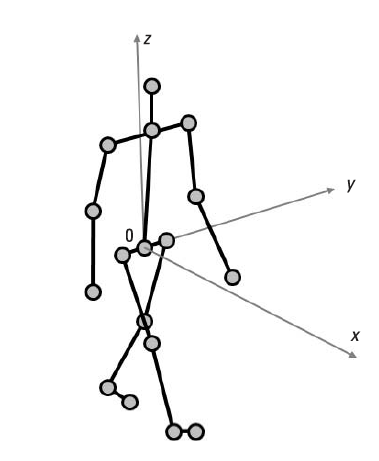
\includegraphics[width=8cm]{Time-frequency analysis-chap3/img/Scatter body model.png}
    \caption{Example of scatter center model for human body.\cite{microdoppler_chen}}
    \label{Humanscatterbody}
\end{figure}


The benefit of such a model is that the received signal can be modelled as the sum of the contributions from the individual points. 
So it's possible to consider the echo received by the N scatter points composing the total body as:

\begin{equation}
s_{r}(t)=\sum_{n} \sigma_{n} s_{T}\left(t-\frac{2 R_{n}}{c}\right)
\label{generalscatterpointreceivedsignal}
\end{equation}

\begin{itemize}
     \item \textbf{$R_{n}$}: is the distance of the n-th point form the radar.

         
    \item \textbf{$s_{T}(t)$}: is a generic signal transmitted by a radar.
         
    \item \textbf{$\sigma_{n}$}: is the RCS contribution of n-th scatter points.
        
\end{itemize}

Focusing on the RCS of a target consisting of N points as in this case, each will result in a phase contribution and amplitude contribution as shown in the following expression (\ref{scattermodeleq}).

\begin{equation}
\sigma_{tot}=\left|\sum_{i=1}^{N} \sigma_{i}\right|^{2} =\left|\sum_{i=1}^{N} \alpha_{i} \exp \left(j \frac{4 \pi}{\lambda} \delta_{i}\right)\right|^{2}
\label{scattermodeleq}
\end{equation}

Where $\alpha_{i}$ is the amplitude contribution of each point and $\delta_{i}$ is the distance between the center of mass of the body and i-th points project on the line of sight. An illustrative example is shown in the figure \ref{ComplexRCS}

\begin{figure}[h!]
    \centering
    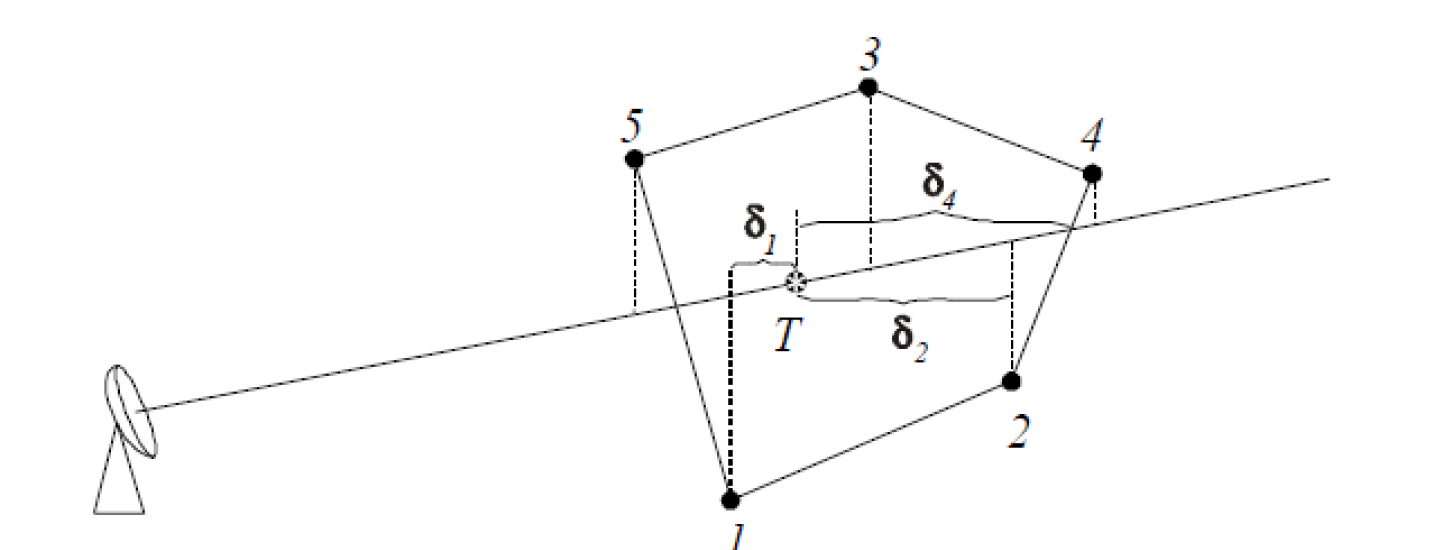
\includegraphics[width=16cm]{Time-frequency analysis-chap3/img/RCS complex body.png}
    \caption{Body composed of 5 different scatter points. \cite{galati_radar}}
    \label{ComplexRCS}
\end{figure}


    
Interested in a continuous wave (CW) radar $s_{T}(t)$ take a form of:

\begin{equation}
s_{T}(t)=e^{j\left(2 \pi f_{0} t+\theta_{0}\right)}
\end{equation}

Taking into account the expression of RCS in \ref{scattermodeleq} and the general formulation of echo received from a target composed by several scatter points \ref{generalscatterpointreceivedsignal}, the backscattered signal became:

\begin{equation}
S_{R}(t)=\sum_{i=1}^{N} \alpha_{i} e^{j \frac{4 \pi}{\lambda} \delta_{i}} e^{j\left[2 \pi f_{0}\left(t-2 \frac{R}{c}\right)+\theta_{0}\right]}
\label{receivesigCW}
\end{equation}

Typically in the CW radar chain the received signal is filtered out by a low pass filter in order to minimize leakage, coming from transmitting antenna, the multipath effect and the clutter coming from unwanted range frequencies. After bandpass transform the first phase term is rejected and in order to estimate the received Doppler frequency, the first derivative of the phase divided by $2\pi$ is performed. So the result is:

\begin{equation}
f_{D}=\frac{1}{2 \pi} \frac{d}{d t} \phi(t)=-\frac{2 v_{r}}{c}
\end{equation}

So it's possible to rewrite the \ref{receivesigCW} highlighting frequencies in the phase term rather than time delay, then the result is:

\begin{equation}
S_{R}(t)=\sum_{i=1}^{M} \alpha_{i} e^{j \frac{4 \pi}{\lambda} \delta_{i}} e^{j\left[2 \pi\left(f_{0}+f_{D}\right) t+\theta_{0}\right]}
\label{CWbackscattered_freq}
\end{equation}



And considering that each point may also have a different radial velocity with respect to the radar, the Doppler frequency of the i-th point can be rewritten as:

\begin{equation}
f_{D_{i}} = -\frac{2 v_{r_{i}}}{c}
\end{equation}

Where $ v_{r_{i}} $ is the radial velocity of the i-th point. So the \ref{CWbackscattered_freq} became:

\begin{equation}
S_{R}(t)=\sum_{i=1}^{M} \alpha_{i} e^{j \frac{4 \pi}{\lambda} \delta_{i}} e^{j\left[2 \pi\left(f_{0}+f_{D_{i}}\right) t+\theta_{0}\right]}
\end{equation}

In the end with this type of signal model it's possible to take into account the different positions of each scatter points composing the total body and also the different velocities that they may have. A brief analysis of the Doppler effect in radar is given in the next section.


\section{Micro-Doppler effect in narrowband radar}
The Doppler effect is used by a radar to measure the radial velocity of targets. As is well known, by measuring the time delay of a signal received from a target, it is possible to calculate the distance at which the target is located. If the target is moving, the frequency of the received signal is used to measure the speed of the target. In addition to the translational motion of the target, the rotational motion of one or more parts of the same body is also considered. In this way, the Doppler contribution due to translation undergoes a modulation due to the rotations of its parts. \\
Approximating the target as a generic scatter point to simplify calculations, if we consider a generic narrowband signal trasmitted by a radar:

\begin{equation}
s(t)=\exp \left(j 2 \pi f_{c} t\right),
\end{equation}

Considering the presence of a generic scatter point at distance $\mathbf{R_{\text {0}}}$ from the radar, moving with radial velocity $v$ and rotating with angular velocity described by a rotation matrix $\mathbf{R_{\text{rotating}}}$, in a 3D model depicted in figure \ref{3dmodel}. Its distance from the radar varies in time according to the following law:

\begin{equation}
\begin{aligned}
R(t) &=\left\|\mathbf{R}_{0}+\mathbf{v} t+\mathbf{R}_{\text {rotating }} \hat{\boldsymbol{r}}_{0}\right\| \\
&=\sqrt{\left(\mathbf{R}_{0}+\mathbf{v} t+\mathbf{R}_{\text {rotating }} \widehat{\boldsymbol{r}}_{0}\right)^{\mathrm{T}}\left(\mathbf{R}_{0}+\mathbf{v} t+\mathbf{R}_{\text {rotating }} \widehat{\boldsymbol{r}}_{0}\right)}
\end{aligned}
\end{equation}

\begin{figure}[h!]
    \centering
    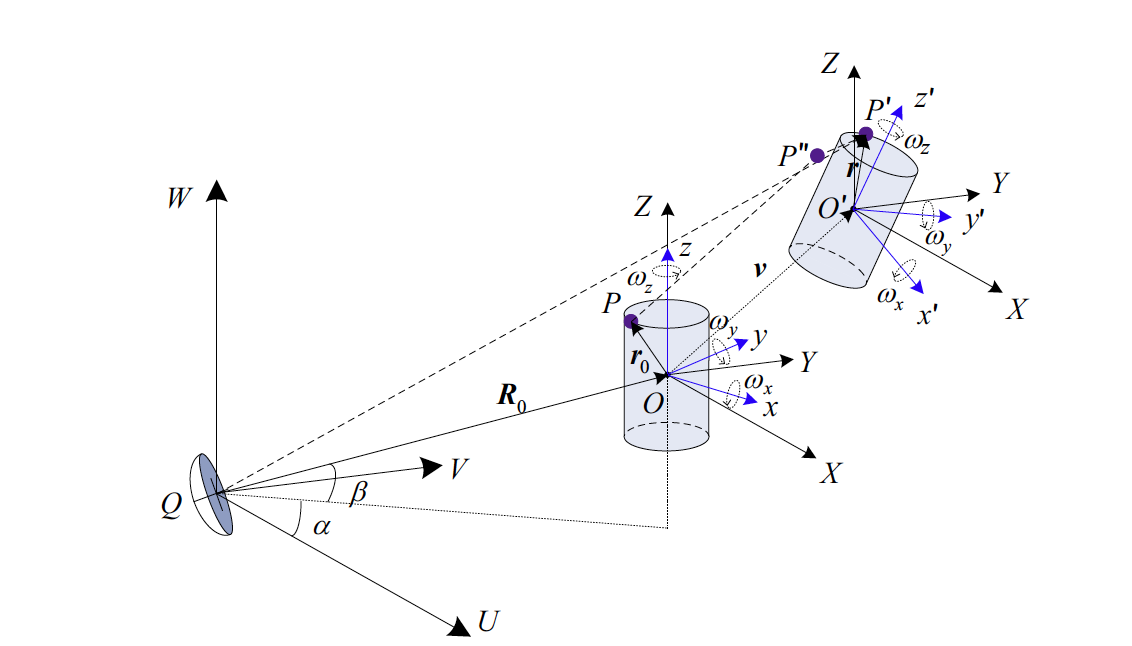
\includegraphics[width=8cm]{Time-frequency analysis-chap3/img/3D model.png}
    \caption{Geometry of 3D model for radar and target.}
    \label{3dmodel}
\end{figure}

Where $\widehat{\boldsymbol{r}}_{0}$ represent the vector of initial position of the scatter point.
The signal backscattered form the generic scatter point become:

\begin{equation}
s(t)=\sigma \exp \left(\mathrm{j} 2 \pi f_{\mathrm{c}}\left(t-\frac{2 R(t)}{c}\right)\right)
\end{equation}

After translating the signal in baseband only the delay component remains i.e. the phase contributions due to the range of target. Computing the instantaneous frequency by taking the first derivative of the phase and dividing it by $2\pi$ the Doppler frequency is obtained:

\begin{equation}
f_{\mathrm{d}}=\frac{1}{2 \pi} \frac{\mathrm{d} \Phi(t)}{\mathrm{d} t}=\frac{2 f_{\mathrm{c}}}{c} \frac{\mathrm{d}}{\mathrm{d} t} R(t)
\end{equation}

\begin{equation}
f_{\mathrm{d}}=\frac{2 f_{\mathrm{c}}}{c}\left[\boldsymbol{v}+\frac{\mathrm{d}}{\mathrm{d} t}\left(\mathbf{R}_{\mathrm{rotating}} \overline{\boldsymbol{r}}_{0}\right)\right]^{\mathrm{T}} \boldsymbol{n} \text {, }
\label{totdoppler}
\end{equation}

Where $\textbf{n}$ is the line of sight unit vector in a far field approximation.\\
Equation \ref{totdoppler} clearly shows the additional Doppler contribution due to the rotation of the scatter point, which in jargon is called the micro Doppler frequency. 
Focusing on this term, considering the time evolution of the rotation matrix, it is possible to show that it represents a 3D rotation matrix, as it is showed in \cite{microdoppler_chen}. This means that it can be expressed using Rodrigues formulas that return the final position of a vector given a rotation angle. In the end, the expression of this term is:

\begin{equation}
f_{\text {micro-Doppler }}=\frac{2 f_{\mathrm{c}} \Omega}{c}\left\{\left[\widehat{\boldsymbol{\omega}}^{\prime 2} \sin (\Omega t)+\widehat{\boldsymbol{\omega}}^{\prime} \cos (\Omega t)\right] \mathbf{R}_{\text {init }} r_{0}\right\}^{\mathrm{T}} n
\end{equation}

Where $\widehat{\boldsymbol{\omega}}^{\prime}$ is the skew symmetric matrix and $ \mathbf{R}_{init }$ is the rotation matrix of initial position of scatter point. Temporal evolution of this therm is showed in figure \ref{mDevolution}, in which three scatter points are considered, one have no micro Doppler frequency hence its contribute is zero (blue line). It is easy to identify the typical sinusoidal pattern where the central Doppler frequency, the one due to the translational speed of the target, is subjected to a modulation due to the rotational speed of the rotating parts on the body.

\begin{figure}[h!]
    \centering
    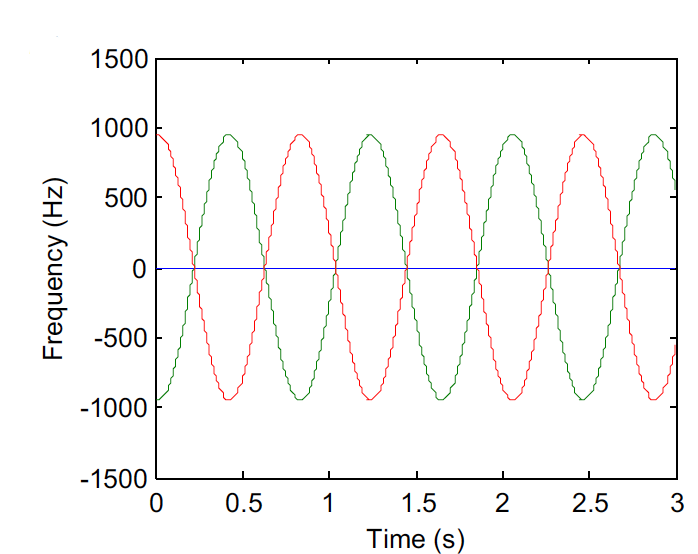
\includegraphics[width=8cm]{Time-frequency analysis-chap3/img/mD effect.png}
    \caption{Temporal evolution of micro Doppler frequency.}
    \label{mDevolution}
\end{figure}

In general, in order to see this effect on the time-frequency plane several constraints are imposed to radar parameters as resolutions. In the case of narrowband radar this effect is emphasised in the time-frequency plane and consequently the tool needed to visualise it is the STFT (Short Time Fourier Transform).
The plot of frequency over time is usually called 'spectrogram'. A general discussion about that is made in next paragraph (3.3). 
There are some differences in the case of a wideband radar, some radar parameters like resolution change, so as will be analysed in detail below this effect is not only emphasised in the time-frequency plane, but can be also observed in the range-time plane under appropriate conditions.











\subsection{The spectrogram}
The instrument that allows the micro-Doppler phenomenon to be observed over frequencies is the spectrogram, it is a plot of frequencies variations over time. In figure \ref{spect_helicopter} is shown an example of a spectrogram of a signal received from an helicopter rotor blades \cite{md_helicopter}. The simple Fourier transform does not allow us to observe the temporal evolution of frequency, but rather to obtain the frequency information content of a signal at a given time instant. 

\begin{figure}[h!]
    \centering
    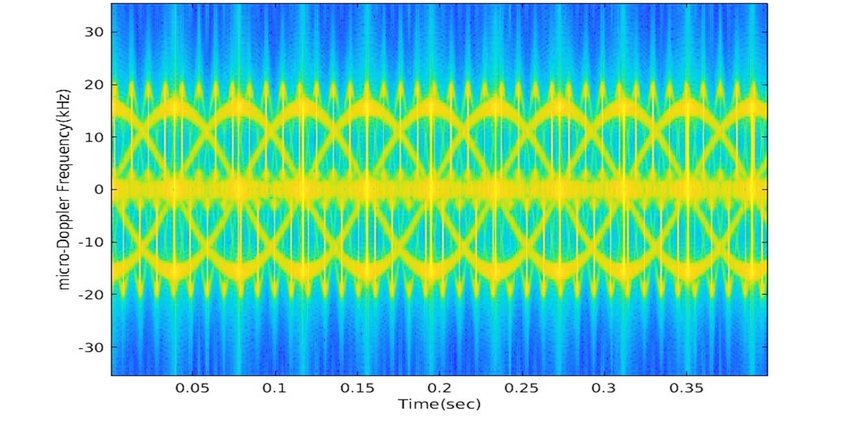
\includegraphics[width=10cm]{Time-frequency analysis-chap3/img/Spectrogram-of-modelled-helicopter-returned-echo.jpg}
    \caption{Spectrogram of helicopter rotor blades.}
    \label{spect_helicopter}
\end{figure}

In order to observe temporal variations in frequency, it is therefore necessary to perform a Fourier transform for each time interval smaller than the total duration of the signal. The instrument that allows this analysis to be carried out is the Short Time Fourier Transform (STFT).

\begin{equation}
\operatorname{STFT}\{x(t)\}(\tau, \omega)=X(\tau, \omega)=\int_{-\infty}^{+\infty} x(t) w(t-\tau) e^{-j \omega t} d t
\end{equation}

Where the considered time interval in which each transformation is made is determined by the length of window $w(t)$. So the choice of a suitable window is critical for time and frequency resolutions. Reasoning about the length of the window $w(t)$: 

\begin{itemize}
     \item \textbf{Increasing the length}: the time during which the signal is observed is longer. Therefore, it is possible to distinguish more different frequencies, resulting in better frequency resolution $ \Delta f$. On the other hand, the variations captured over time are less, resulting in a lower temporal resolution $\Delta t$ 

         
    \item \textbf{Decreasing the length}: the time during which the signal is observed is smaller. Therefore, it is possible to capture more variations over time, resulting in a higher time resolution $ \Delta t$ . As consequence the frequency resolution $\Delta f$ is smaller.
    
\end{itemize}


Having analysed the effects of window length on time and frequency resolution, it is now possible to look at a typical example of a window being used.
Reasoning about its spectrum, usually the Hamming window is used to obtain a good trade off between the ratio of main lobe and side lobes and the width of the main lobe. Difference between rectangular window and raised cosine window (Hamming) is shown in figure \ref{rect_vs_hamming}.

\begin{figure}[h!]
    \centering
    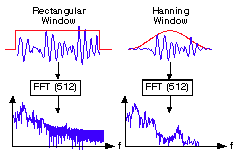
\includegraphics[width=10cm]{Time-frequency analysis-chap3/img/Difference among window.png}
    \caption{Rectangular window vs Hamming window.}
    \label{rect_vs_hamming}
\end{figure}



Then the spectrogram is obtained by squaring the modulus of the STFT.

\begin{equation}
\text { Spectrogram }\{x(t)\}(\tau, \omega)=|X(\tau, \omega)|^{2}
\end{equation}

In figure \ref{STFTgraph} is showed graphically the procedure done by STFT.

\begin{figure}[h!]
    \centering
    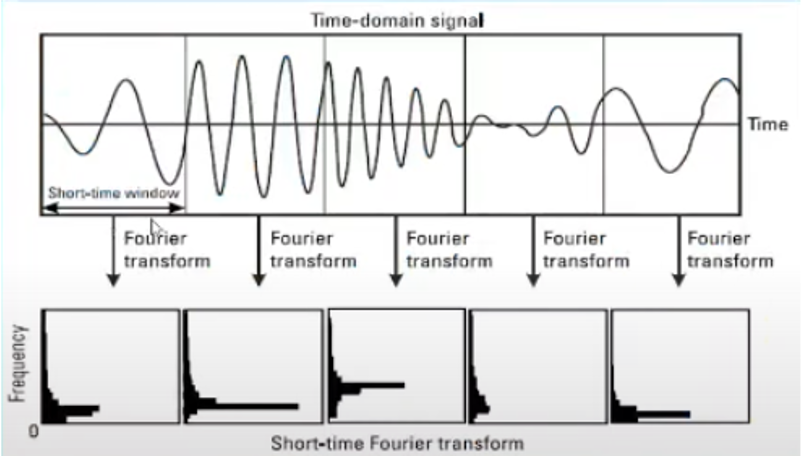
\includegraphics[width=10cm]{Time-frequency analysis-chap3/img/STFTexample.png}
    \caption{STFT of a generic signal.}
    \label{STFTgraph}
\end{figure}

\section{Micro-Doppler effect in wideband radar}
More attention is now given to the analysis of the wideband case, which is of main interest as the FMCW radar belongs to this category.\\
The use of a wideband radar brings many benefits and is chosen especially considering the possibility of obtaining a high band-time product. In addition, unlike a narrowband radar, the energy is spread over a much wider range, resulting in a very low peak transmitted power. This reduces costs, difficulties and greatly increases range resolution as discussed in detail in Chapter 2.\\ In general, radars with these characteristics are more sensitive to the micro-Doppler effect, as they are able to pick up smaller differences in time and frequency. As mentioned in the previous paragraphs, in this case the micro-Doppler effect can already be observed in the range-time plane under appropriate conditions, due to the larger bandwidth. \\
A typical linear frequency modulated radar represents a coherent system, so the signal received by the target undergoes coherent integration of all the ramps sent on target during the dwell time. From this point of view it is convenient to consider the total radar time divided into fast and slow time, as suggested in \cite{chen_chinese}:

\begin{equation}
t=t_{s}+t_{f}
\label{fasttimeslowtime}
\end{equation}



\begin{itemize}
     \item \textbf{$t_{s}$}: is the slow time associated with slow sampling that occurs every ramp repetition interval that making a parallelism with a pulsed radar, it's possible to call this Pulse Repetition Interval (PRI). $t_{s}$ is also called interpulse time.

         
    \item \textbf{$t_{f}$}: is the fast time, associated with the fast sampling that takes place within each PRI. This time is also called intrapulse time.
    
\end{itemize}

Inserting \ref{fasttimeslowtime} in \ref{reflectedsigfinal} the generic backscattered signal from a target can be rewrite in function of slow and fast time:

\begin{equation}
s\left(t_{f}, t_{s}\right)=\sigma u\left(\frac{c+v_{r}}{c-v_{r}} t_{f}-\frac{2 R\left(t_{s}\right)}{c-v_{r}}\right) \exp \left[j \omega_{0}\left(\frac{c+v_{r}}{c-v_{r}} t_{f}-\frac{2 R\left(t_{s}\right)}{c-v_{r}}\right)\right]
\label{reflectedsig_slow_fast_time}
\end{equation}

Considering the range also as function of fast time and not only of slow time:

\begin{equation}
R\left(t_{s},t_{f}\right)=R_{0}-v_{r} t_{s}-v_{r} t_{f}
\label{range_slow_fast}
\end{equation}

Substituting \ref{range_slow_fast} in \ref{reflectedsig_slow_fast_time}:

\begin{equation}
\begin{array}{c}
s\left(t_{f}, t_{s}\right)=\sigma u\left(\frac{c+v_{r}}{c-v_{r}} t_{f}-\frac{2 R\left(t_{s}\right)}{c-v_{r}}\right) \exp \left(j \omega_{0} t_{f}\right) \exp \left(-j \omega_{0} \frac{2 R_{0}}{c-v_{r}}\right) \\
\cdot \exp \left(j \omega_{0} \frac{2 v_{r}}{c-v_{r}} t_{f}\right) \exp \left(j \omega_{0} \frac{2 v_{r}}{c-v_{r}} t_{s}\right)
\end{array}
\label{completeformula}
\end{equation}


In general, working with such a signal in radar applications is rather complicated.  The different translation terms in the signal due to distance and speed of the target are not particularly harmful to the envelope since they are simple translations on the time axis. On the other hand, they can create non-negligible problems on the signal phase, e.g. by making it difficult to estimate the real distance or speed of the target.

In the formula \ref{completeformula} particular attention is paid to the last two exponential terms. They represent:

\begin{itemize}
     \item \textbf{The intrapulse Doppler effect}: due to the penultimate exponential term (function of fast time), its main effect is to deviate the centre of the spectrum of the received echo.
     Theoretically, the received echo spectrum, after dechirp operation, is a sinc function and within the pulse repetition interval is shifted by an amount equal to the distance travelled by the target during the fast time. As we will see later in the simplified models, usually considering the translation speed of a target quite contained and the fast time very small, this effect can be considered negligible.

         
    \item \textbf{The interpulse Doppler effect}: due to the last exponential term (function of slow time), whose main effect is to change the initial phase of each pulse. In fact, it is typically taken into account to estimate the speed of an object by performing the Fast Fourier Transform of M successive pulses. Since the space travelled by the target during slow time is appreciable compared to the phase shift that occurs during fast time.
    
\end{itemize}

In general, two different models with two different and gradual approximations are often used to simplify formulation \ref{completeformula}:

\begin{itemize}
     \item \textbf{The first-order approximate model}: this model makes a single, simple approximation: the radial velocity of the target is considered to be much smaller than the speed of light. 
     \begin{equation}
        \left(c-v_{r}\right) \sim c
     \end{equation}
     The received echo from target with only translation velocity (formula \ref{completeformula}) in this case become:
     
     \begin{equation}
     \begin{aligned}
     s\left(t_{f}, t_{s}\right)=& \sigma         u\left(t_{f}-\frac{2\left(R\left(t_{s},t_{f}\right) \right)}{c}\right) \exp\left(j \omega_{0} t_{f}\right) \exp \left(-j \omega_{0} \frac{2             R_{0}}{c}\right) \\
     & \cdot \exp \left(j \omega_{0} \frac{2 v_{r}}{c} t_{f}\right) \exp \left(j         \omega_{0} \frac{2 v_{r}}{c} t_{s}\right)
     \end{aligned}
     \label{firstordermodelformula}
     \end{equation}

     
     Consequently, it is the model that have more phase terms and makes the treatment slightly more complicated. Nevertheless, it is well suited in radar wideband situations and allows one to observe and evaluate the effects that occur during the pulse integration time. It is also the more accurate model that take into account all the effect of target moving during the intrapulse time, is therefore more in line with reality.

         
    \item \textbf{The stop-go approximate model}: This is the most simplified model, in fact it's a further approximation of the previous model. In addition to the velocity approximation already made, also the product between the radial velocity of the target and the fast time is considered to be approximately very small and therefore negligible. Under this assumption it is as if the target remains stationary for the duration of the intrapulse time and begins to move at each PRI instant.
    \begin{equation}
    \left(v_{r} t_{f}\right) \sim 0
    \end{equation}
    
    The received echo from target with only translation velocity ( \ref{completeformula}) in this case become:
    
    \begin{equation}
    s\left(t_{f}, t_{s}\right)=\sigma u\left(t_{f}-\frac{2 R\left(t_{s}\right)}{c}\right) \exp \left(j \omega_{0}\left(t_{f}-\frac{2 R\left(t_{s}\right)}{c}\right)\right)
    \end{equation}
    
    It's important to note that now the range equation depends only on the slow time $t_{s}$ and its expression is:
    
    \begin{equation}
    R\left(t_{s}\right)=R_{0}-v_{r} t_{s}
    \label{range_slow_fast_time}
    \end{equation}
\end{itemize}

So the \ref{completeformula} became:

\begin{equation}
     \begin{aligned}
     s\left(t_{f}, t_{s}\right)=& \sigma         u\left(t_{f}-\frac{2 R\left(t_{s}\right) }{c}\right) \exp\left(j \omega_{0} t_{f}\right) \exp \left(-j \omega_{0} \frac{2             R_{0}}{c}\right) \\
     & \cdot  \exp \left(j         \omega_{0} \frac{2 v_{r}}{c} t_{s}\right)
     \end{aligned}
     \label{stopgomodelformula}
\end{equation}

The stop-go model can be used if the speed of the target is not too high, and the duration of each pulse is not too long. In the specific case of an FMCW radar, given the long time duration of each ramp (compared to the ones of pulsed radar) and the large bandwidth available, it is not always possible to neglect the target shifts that occur during the intrapulse time, i.e. the fast time. For this reason, the first-order model is usually used in the case of wideband radar and a stop-go model is used in the case of narrowband radar with low-speed targets. In the following sub-sections it's considered the use of the two signal models just seen on a chirp signal in order to highlight the differences and what is lost by deciding to use one model at the expense of the other.

\subsection{Dechirp operation in LFM}
A typical linear frequency modulation (LFM) signal has the following expression \ref{chirpsignal}, it is often called chirp signal:

\begin{equation}
s(t)=\operatorname{rect}\left(\frac{t}{T_{c}}\right) \cdot \exp \left(j 2 \pi\left(f_{c} t+\frac{1}{2} \mu t^{2}\right)\right)
\label{chirpsignal}
\end{equation}

Where the typical values of FMCW radar are:

\begin{itemize}
     \item \textbf{$T_c$}: is the duration of each chirp, i.e. the PRI;
         
    \item \textbf{$\mu$}: is the frequency shift per unit time i.e. the slope;
    
    \item \textbf{$f_c$}: is the centre frequency;
\end{itemize}

The typical graph of a chirp signal is shown in the figure \ref{chirpimg}.

\begin{figure}[h!]
    \centering
    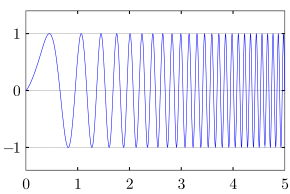
\includegraphics[width=8cm]{Time-frequency analysis-chap3/img/chirpsig.png}
    \caption{Chirp signal.}
    \label{chirpimg}
\end{figure}

For simplicity, it is considered the case where there is a fixed target at distance $R$ from the radar, so the received signal becomes:

\begin{equation}
s_{r}(t)=\sigma \operatorname{rect}\left(\frac{t-2 R / c}{T_{c}}\right) \cdot \exp \left(j 2 \pi\left(f_{c}\left(t-\frac{2 R}{c}\right)+\frac{1}{2} \mu\left(t-\frac{2 R}{c}\right)^{2}\right)\right)
\end{equation}


In the typical chain of FMCW radar the received signal is subjected to an operation called 'dechirp'. Making an analogy with pulse radar, the same operation is done with a matched filter.
Dechirping in FMCW radar is done by mixing the signal received from the target and the transmitted reference signal. The general expression of the reference signal is:

\begin{equation}
s_{r e f}(t)=\operatorname{rect}\left(\frac{t-2 R_{r e f} / c}{T_{r e f}}\right) \cdot \exp \left(j 2 \pi\left(f_{c}\left(t-\frac{2 R_{r e f}}{c}\right)+\frac{1}{2} \mu\left(t-\frac{2 R_{r f}}{c}\right)^{2}\right)\right)
\end{equation}

Where $R_{r e f}$ is the distance associated to the considered reference delay.
The output of 'dechirp' operation is the product of received signal $s_{r}$ with complex conjugate of reference $s_{r e f}$, it is called 'beat' signal and the result is:

\begin{equation}
\begin{array}{l}
s_{b}(t)=s_{r}(t) s_{r e f}^{*}(t) \\
=\sigma \operatorname{rect}\left(\frac{t-2 R / c}{T_{p}}\right) \\
\quad \cdot \exp \left(j\left(-\frac{4 \pi}{c} \mu\left(t-\frac{2 R_{r ef}}{c}\right) R_{\Delta}-\frac{4 \pi}{c} f_{c} R_{\Delta}+\frac{4 \pi \mu}{c^{2}} R_{\Delta}^{2}\right)\right)
\end{array}
\label{beatsignal}
\end{equation}
\\
Where $R_{\Delta}$ is the difference between the distance of target e the distance associated to the reference delay of reference signal.
For simplicity $R_{r e f}$ and corresponding reference delay are considered equal to zero, and so the \ref{beatsignal} turn into:
\begin{equation}
s_{b}\left(t\right)=\sigma \operatorname{rect}\left(\frac{t-2 R / c}{T_{c}}\right) \cdot \exp \left(j\left(-\frac{4 \pi}{c} \mu R t-\frac{4 \pi}{c} f_{c} R+\frac{4 \pi \mu}{c^{2}} R^{2}\right)\right)
\label{finalbeat}
\end{equation}

In order to better visualize the result, in figure \ref{Dechirpfigure} is shown the operation on a frequency-time plane.

\begin{figure}[h!]
    \centering
    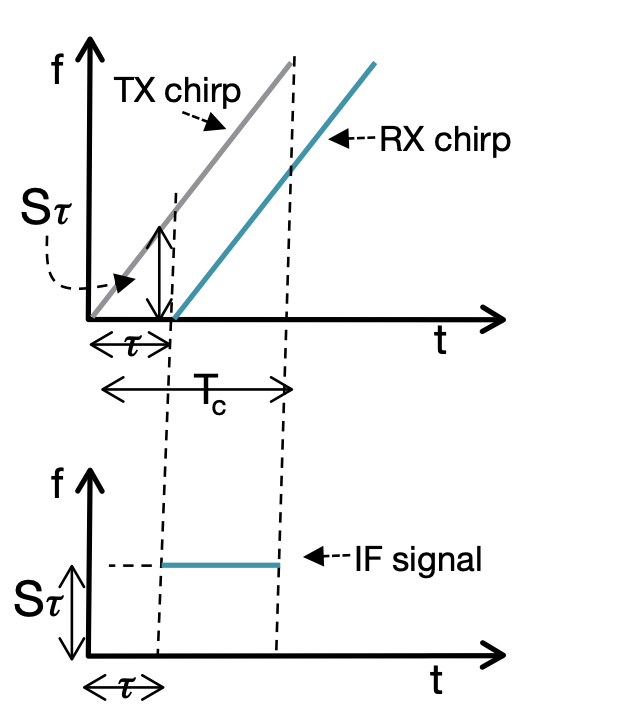
\includegraphics[width=5cm]{Time-frequency analysis-chap3/img/dechirp.png}
    \caption{Dechirp operation.}
    \label{Dechirpfigure}
\end{figure}


It's easy to notice that as a result of dechirp operation the original wideband signal is now transformed into a narrowband signal. This is a great benefit in terms of component requirements. Although a very wide bandwidth is used for transmission, an inferred bandwidth is required at the receiving end. In fact, as already seen in Chapter 2 one of the main benefits of the FMCW radar is just that.
Focusing on the phase terms in the exponential of \ref{finalbeat}:


\begin{itemize}
     \item \textbf{The first term}: is constant only if the target is stationary ($R$ fixed). If the target starts to move, the range becomes time-varying and takes on a different value with each pulse received. It is therefore a variable function of the target range;
         
    \item \textbf{The second term}: is called sideling term and is considered as an additive noise to the first phase term;
    
    \item \textbf{The third term}: is called residual video phase (RVP) and like the previous one is an additional noise;
\end{itemize}

The spectrum of the beat signal in \ref{finalbeat} is:


\begin{equation}
S_{b}(f)=\sigma T_{c} \operatorname{sinc}\left(T_{c}\left(f+\frac{2 \mu}{c} R\right)\right) \cdot \exp \left(-j \frac{4 \pi}{c} f_{c} R -j \frac{4 \pi f}{c} R+j \frac{4 \pi \mu}{c^{2}} R^{2}\right)
\end{equation}

The peak value of the sinc is centered on the frequency $
f=-2 \mu R / c
$
and for that value of frequency the exponential values of sideling and RVP terms can be suppressed by multiplying $S_{b}(f)$ by:

\begin{equation}
\operatorname{S}_{\mathrm{RVP}}(f)=\exp \left(-j \frac{3 \pi f^{2}}{\mu}\right)
\end{equation}

In fact the sum of RVP phase term and sideling phase term for $
f=-2 \mu R / c
$
, as detailed described in \cite{chen_chinese}, is:

\begin{equation}
\frac{4 \pi \mu}{c^{2}} R^{2}-\frac{4 \pi f}{c} R=\frac{3 \pi f^{2}}{\mu}
\end{equation}

\subsection{mD with Stop-go model}

Considering the 'Stop-go' model approximation of received signal from target in \ref{stopgomodelformula}, the LFM signal in function of slow time and fast time is:

\begin{equation}
s_{r}\left(t_{f}, t_{s}\right)=\sigma \operatorname{rect}\left(\frac{t_{f}-2 R\left(t_{s}\right) / c}{T_{c}}\right) \cdot \exp \left(j 2 \pi\left(f_{c}\left(t_{f}-\frac{2 R\left(t_{s}\right)}{c}\right)+\frac{1}{2} \mu\left(t_{f}-\frac{2 R\left(t_{s}\right)}{c}\right)^2\right)\right)
\end{equation}
\\
Considering the target moves with radial velocity $v_{r}$ and rotates with angular velocity $\Omega$, the range as a function of slow time is:

\begin{equation}
\begin{aligned}
R\left(t_{s}\right) &=\left\|\mathbf{R_{\text {0}}}+\mathbf{v} t_{s}+\mathbf{R}_{\text {rotating }}\left(t_{s}\right) \mathbf{\widehat{r}_\text{0}}\right\| \\
&=\sqrt{\left(\mathbf{R}_{0}+\mathbf{v} t_{s}+\mathbf{R}_{\text {rotating }}\left(t_{s}\right) \mathbf{\widehat{r}_\text{0}}\right)^{\mathrm{T}}\left(\mathbf{R_{\text{0}}}+\mathbf{v} t_{s}+\mathbf{R}_{\text {rotating }}\left(t_{s}\right) \mathbf{\widehat{r}_\text{0}}\right)}
\end{aligned}
\end{equation}

As usual, for simplicity the reference signal is considered with a null delay and as consequence the distance $R_{ref}$ associated to that delay is zero.
After the dechirp operation, as described in the precedent subsection, is produced a beat signal as follow:


\begin{equation}
\begin{aligned}
s_{b}\left(t_{f}, t_{s}\right)=& s_{r}\left(t_{f}, t_{s}\right) s_{r e f}^{*}\left(t_{f}, t_{s}\right) \\
=& \sigma \operatorname{rect}\left(\frac{t_{f}-2 R 
\left(t_{s}\right) / c}{T_{c}}\right) \\
& \cdot \exp \left(j\left(-\frac{4 \pi}{c} \mu t_{f}
R\left(t_{s}\right)-\frac{4 \pi}{c} f_{c} R\left(t_{s}\right)+\frac{4 \pi \mu}{c^{2}} R\left(t_{s}\right)^{2}\right)\right)
\end{aligned}
\label{beatstopgomodel}
\end{equation}

Taking the Fourier transform in the fast time, i.e. $t_{f}$, and suppressing the annoying phase terms, i.e.  the sideling and RVP terms, the spectrum of the beat signal is:

\begin{equation}
S_{b}\left(f_{f}, t_{s}\right)=\sigma T_{c} \operatorname{sinc}\left(T_{c}\left(f_{f}+\frac{2 \mu}{c} R\left(t_{s}\right)\right)\right) \cdot \exp \left(-\mathrm{j} \frac{4 \pi}{c} f_{c} R\left(t_{s}\right)\right)
\end{equation}

It is possible to observe how the phase is modulated by $R(t_{s})$ and thus determines the characteristic effect of the micro-doppler described in the previous paragraph and so it is observable in the time-frequency plane. While the sinc peak also shifts as a function of $R(t_{s})$. With a narrowband radar the variations induced by the micro-Doppler were observable only on the phase, instead using a wideband radar these variations become visible also on the sinc peak. This is due to the fact that bandwidth is higher and so the range resolution is higher. It is therefore possible to state that by using a wideband radar it is possible to observe the micro-Doppler effect also on the Range-Slow Time plane and not only on the Time-Frequency plane.

\subsection{mD with First-order model}
Under the conditions of First-order model, the displacement that occurs of the target during fast time can no longer be neglected, in order to observe these variations, the radar range equation is consider as in \cite{chen_chinese}:
\begin{equation}
R(t_{f}) = R_{0} - v_{r} t_{f}
\label{fast_range}
\end{equation}

In \ref{fast_range} for the sake of simplicity only the radial movement of target respect to radar is considered and only the fast time is considered, in order to evaluate the error introduced by using the Stop-go model. In fact the difference among the two model (the Stop-go and the First-Order models) is in the range equation:
\begin{equation}
    R(t_{s},t_{f}) - R(t_{s}) = v_{r}t_{f}
    \label{modeldiffrange}
\end{equation}
Where in the left side of the equation \ref{modeldiffrange} the first term is the range equation under the assumptions of the First-order model, and the second term is the range equation under the assumptions of Stop-go model.
In this case the received LFM signal from that target is:

\begin{equation}
s_{r}\left(t_{f}\right)=\sigma \operatorname{rect}\left(\frac{t_{s}-2 R(t_{f})/ c}{T_{c}}\right) \cdot \exp \left(\mathrm{j} 2 \pi\left(f_{c}\left(t_{f}-\frac{2 R(t_{f})}{c}\right)+\frac{1}{2} \mu\left(t_{f}-\frac{2 R(t_{f})}{c}\right)^{2}\right)\right)
\end{equation}

As usual the dechirp is done with the reference transmitted signal where for simplicity the reference delay is again considered null. The beat signal is then obtained:

\begin{equation}
\begin{aligned}
s_{b}\left(t_{f}\right)=& s_{r}\left(t_{f}\right) s_{r e f}^{*}\left(t_{f}\right) \\
=& \sigma \operatorname{rect}\left(\frac{t_{f}-2 R(t_{f}) / c}{T_{c}}\right) \cdot \exp \left(j\left(-\frac{4 \pi}{c} \mu t_{f} R_{0}-\frac{4 \pi}{c} f_{c} R_{0}+\frac{4 \pi \mu}{c^{2}} R_{0}^{2}\right)\right) \\
& \cdot \exp \left(j\left(-\frac{4 \pi \mu v_{r} t_{f}^{2}}{c}+\frac{4 \pi f_{c} v_{r} t_{f}}{c}\right)\right) \exp \left(j\left(-\frac{8 \pi \mu R_{0} v_{r} t_{f}}{c^{2}}+\frac{4 \pi \mu v_{r}^{2} t_{f}^{2}}{c^{2}}\right)\right)
\end{aligned}
\end{equation}


As described in \cite{chen_chinese} the last exponential term is negligible because is more small in comparison to the others. Calculating the instantaneous frequency of this signal by deriving its phase respect to $t_{f}$ and dividing it by $2\pi$ we obtain:

\begin{equation}
f=-\frac{2 \mu}{c} R_{0}+\frac{2 v_{r}}{\lambda}+\frac{4 \mu}{c} v_{r} t_{f}
\label{instafreq}
\end{equation}
It is important to remark this instantaneous frequency coming from the beat signal related to the echoes received by the target. From this measurement, all three terms that make up the frequency will be analysed in the next section and the effect of cell migration will be measured.

\section{Range cell migration and broadening}
%inserire cosa va ad inficiare l'effetto di migrazione della cella, integrazione coerente tipica di questi radar e l'immagine micro doppler sul piano tempo frequenza
The cell migration effect can be of fixed or variable nature, in order to be clear it's possible to distinguish two different cases:
\begin{itemize}
     \item \textbf{The fixed cell migration}: it is due to the case in which the radial velocity of target does not depend on time. Or more in general it is due to all contributions that are fixed in time and deviate the frequency of the beat signal. This means that if we neglect the third term of \ref{instafreq} and the target moves at a constant speed during processing, the peak of the beat signal spectrum will always be the same in the fast time interval, thus not resulting in variable range migration. Then will be a fixed error on the distance measurement that can be corrected by estimating the Doppler frequency associated to the radial velocity of target. This type of error does not depend on the time taken to perform coherent integration of the signals received from the target. If we observe a target at $4\; m$ far from the radar and with a constant velocity that result in a shift of $1 \;m$ from the real position in range-slow time diagram it's possible to see a fixed line as in picture \ref{fixed_range_slow_time_fig};
     \begin{figure}[h!]
     \centering
     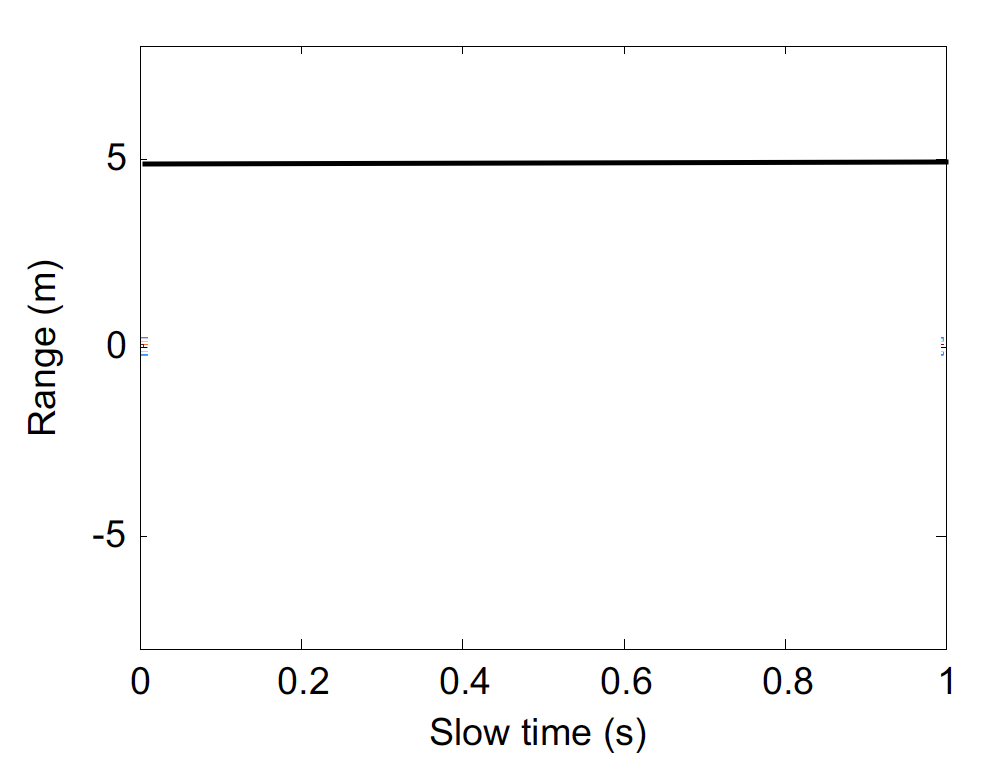
\includegraphics[width=8cm]{Time-frequency analysis-chap3/img/fixed range-slow time.png}
     \caption{Range-Slow time plot of target with constant velocity and no cell migration.}
     \label{fixed_range_slow_time_fig}
     \end{figure}

         
    \item \textbf{The variable cell migration}: The effect of variable cell migration is what interests us most in the case of a target consisting of a main body containing some rotating parts. The radial velocity of rotating part is not constant over time determining a range variation that is also variable with time. So at each slow time instant the range variation due to the radial velocity of a rotating object will be different, but at same time it will be periodic, i.e. sinusoidal. So we can distinguish a pattern in the range-slow time plane. In figure \ref{var_range_slow_time_fig} is shown the range-slow time plot of a  target with rotational movements at $3\;m$ from radar. It's possible to observe a range variations of about $12\;m$ from its centre of rotation due to the rotational movements.
    \begin{figure}[h!]
     \centering
     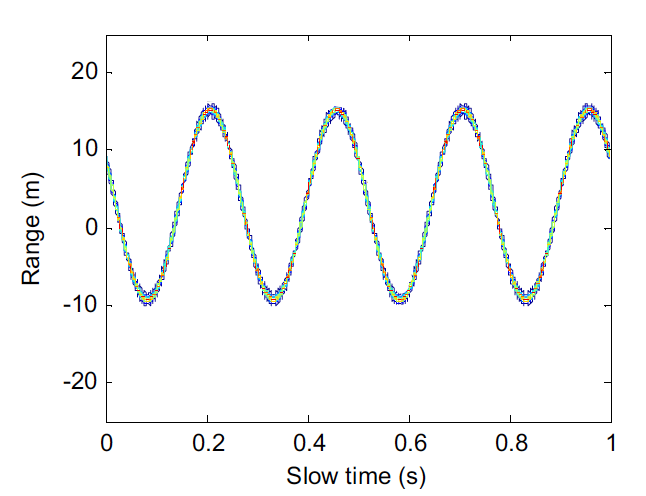
\includegraphics[width=8cm]{Time-frequency analysis-chap3/img/var_slow_time.png}
     \caption{Range-Slow time plot of a rotating point with no translation and cell migration.}
     \label{var_range_slow_time_fig}
     \end{figure}
    
\end{itemize}

As we expect to see in formula \ref{instafreq}, the frequency of received signal is composed by a first term related to the distance of target and two other terms related to the relative motion of the target respect to the radar. The second term is the intrapulse Doppler contribution related to the radial velocity of the target, neglected in the case of the simple Stop-go model. In the simplest model only the Doppler effect on the interpulse is considered, i.e. during the slow time. Now the Doppler effect is consider only during the fast time to evaluate its contribution. The last term is the value that causes the broadening of the peak in the spectrum of the beat signal, as described in \cite{chen_chinese}. The amount of spectrum broadening is directly proportional to its value, in general its absolute value is small compared to the other two terms. The reason why its effect is only a 'broadening' of the spectrum is due to the fast time dependency, each integrated pulse during the coherent integration phase will have a slightly different position. This effect is like to sum up different sinc functions centered 'almost' on the same position. Considering that the fast time is the time during each pulse in which it's possible to perform the FFT of the beat signal and estimate its frequency, as described in detail in \cite{2Dprocessing_fmcw}. Fast time interval is so small in comparison with the slow time interval. To better visualize the fast time interval in figure \ref{txandrxrampintervals} it is denoted as $T - \tau$, where $T$ is the chirp duration (PRI) and $\tau$ is the delay of the received echo.

\begin{figure}[h!]
    \centering
    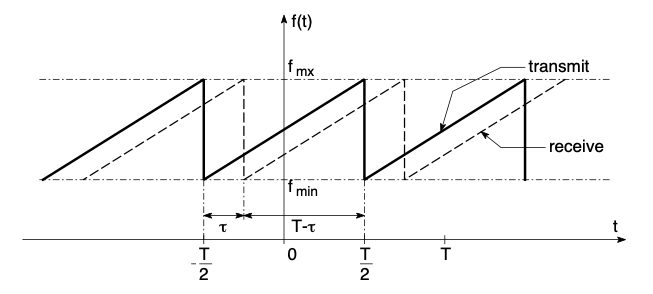
\includegraphics[width=10cm]{Time-frequency analysis-chap3/img/Tx and rx FMCW ramps.png}
    \caption{Time intervals on transmitted and received ramps.}
    \label{txandrxrampintervals}
\end{figure}

 In the case of a narrowband radar the duration of a pulse is very small and consequently the $v_{r}t_{f}$ product becomes incredibly small and certainly negligible. The doubt as to whether or not this contribution can be neglected rises in the case of an X-band wideband FMCW radar where typical ramp durations are around 1 ms.  Using a numerical example, it is possible to calculate how much the terms of the \ref{instafreq} are worth.\\ 
\subsection{Target with only translation}
Considering a FMCW radar and a target with the following parameters: 
 
\begin{itemize}
    \item Bandwidth: $B = 750\; MHz$,
         
    \item Ramp duration: $T_{c} = 1\; ms$,
    
    \item Slope: $\mu = 750\; GHz/s$,
    
    \item Center frequency: $f = 9\; GHz$,

    \item Target distance: $R = 1000\; m$,
    
    \item 2-way delay from $R$: $\tau = 6.67 \;\mu s $,
    
    \item Fast time interval: $T_{c} -\tau = 0.993 \; ms $,
    
    \item Target velocity: $v_{r} = 70 \; km/h$.

\end{itemize}

In this case the three term of the instantaneous frequency \ref{instafreq} are:
 
\begin{equation}
   f = -\frac{2 \mu}{c} R_{0}+\frac{2 v_{r}}{\lambda}+\frac{4 \mu}{c} v_{r} t_{f} = -500 + 1.167 +0.193\, KHz
    \label{firstordershift}
\end{equation}

Usually the last term contribution is neglected because as it is possible to see it is so small in relation to the first and second terms. In fact, dividing it for $-2\mu/c$ the variation in range due to it is only $3.8 \; cm$. Remembering that we are using an FMCW radar and the frequency is related to the range in a linear way:

\begin{equation}
    R = \frac{c f}{2 \mu} 
\end{equation}

So, turning the frequency shift in distance values, the range variations from the real target distance is: 
\begin{equation}
    R_{var} = R_0 - \frac{c v_{r}}{\lambda \mu} -2v_r t_f
    \label{rangevar}
\end{equation} 
The second term of \ref{rangevar} is the most important, it is the so-called intra Doppler effect and its value is much greater than the others. It is usually sufficient to take only it into account to quantify the migration.
As seen in \ref{rangevar} where c is the light speed, using a Stop-go model compared to the First-order model results in an error in range measurement of each ramps of: 
\begin{equation}
    R_{err} = R_0 - R_{var} = \frac{c v_{r}}{\lambda \mu} + 2v_r t_f = 0.27\; m
    \label{rangerror_stopgo}
\end{equation} 

Interesting only in the fast time interval, without considering the migration effect that occurs in slow time. (Base assumption made in \ref{fast_range} to evaluate the micro Doppler effect only present in the First-order model)
From \ref{rangerror_stopgo} it's possible to see that in addition to the sinc-shifting effect due to the radial velocity, there is also a sinc-widening effect resulting from coherent processing and due to the last term. 
As this term depends on the fast time interval, i.e. $t_{f}$ varies with the target distance, so if the target moves the coherent integration will be done on slightly shifted sincs. The result of integration is a slightly lager sinc.
The effect is therefore a deterioration of the range resolution.\\ Considering the parameters of the previous example, the range resolution of the radar used is:
\begin{equation}
    \Delta R = \frac{c}{2B} = 0.2\; m
    \label{resolutionex}
\end{equation}

This equation shows that the size of each range cell is $ 0.2\; m$. The $R_{err}$ in the case described before is greater than the range cell dimension, consequently it means that migration occurs during fast time, but is a type of fixed migration which does not cause problems with the coherent integration of M ramps. For any value of $R_{err}$ less than the size of a range cell, no cell migration occurs during the fast time interval. It is therefore possible to use a Stop-go model even in the case of a wideband radar as long as the following relationship is satisfied:

\begin{equation}
    R_{err} < \Delta R = \frac{c}{2 B}
    \label{stopgo_condition}
\end{equation}

If this condition is not met, in general the radar make an error in distance measurement equal to $R_{err}$. In addition to the range measurement error also the effective resolution of the radar will no longer be the theoretical resolution, due to the term $2 v_r t_f$, as explained before the peak of spectrum of beat signal is not only in a wrong position but it is also broader.
It is important to emphasise two important aspects:
\begin{itemize}
     \item What has just been seen applies to a target that translates without having rotating parts and so considering the radial velocity fixed. In this case the only broadening term is the one dependant on the fast time, i.e $2 v_r t_f$ while the shifting term is constant over time. (The case of cell migration of rotating object will be analyzed in the following section). In this case the effect refers to figure \ref{fixed_range_slow_time_fig} where the broadening time dependant term is so small and not visible, if it had been larger it would have resulted in a slope of the line seen in that figure;
         
    \item The migration effect analysed is the one occurring during fast time, it is important to distinguish it from the same effect occurring during slow time that depend on the time of observation, i.e. the dwell time. (It is taken into account by the stop-go model, the term $v_{r}t_{s}$ is not neglected.);

\end{itemize}

The last concept is the most important to understand that what we have just seen does not clarify if the cell migration effect occurs in its totality, it clarifies if this effect occurs in the short period of the fast time. It therefore tells us whether it is possible to use the stop-go model in the case of a wideband radar by the condition \ref{stopgo_condition}. Then it is a separate issue to check whether the cell migration effect occurs during the slow time and therefore during the whole integration time. The cell migration during slow time, if present, is taken into account by the terms of the Stop-go model.\\
The slow time interval is practically the duration of the dwell time, and therefore it is much longer than the fast time interval. Ideally, the fast time interval can be at most equal to the PRI.
Consequently, during an entire dwell time, using a wideband radar very often results in cell migration if the time of observation is sightly large, because the target really change cell during a long observation.
In fact, in case of coherent integration of M different pulses within a longer dwell time, the difference of peaks positions of each sinc associated to each beat signal is no more 'slightly' and the broadening becomes much more important and even the target will occupy several radar cells in range. This phenomenon is called in literature as 'Cell Migration Effect'.\\
Having clarified which type of cell migration is involved in the case of the two models considered, the case of a static but rotating point target is now considered and the effects on migration are analysed.
\subsection{Target with only rotations}
The effect of using the Stop-go model rather than the First-order model is analysed now in the more interested case where the target has only rotating parts. In this case the range equation of a scatter point that rotates around a center with amplitude $\rho$, as described in \cite{chen_chinese}, is:

\begin{equation}
R\left(t_{s},t_{f}\right)=R_{0}+\rho \cos \left(\Omega (t_{s}+t_{f})+\theta_{0}\right) - v_{r} t_{f}
\label{rotaionfirstorder}
\end{equation}

Where $R_{0}$ is the distance from the radar to center of rotation, the second term is the projection of the rotating scatter point on the line of sight of radar where $\rho$ is the amplitude of the rotation. The third term is null because for simplicity we consider only the rotational movements, no translations are present. So the range equation doesn't depend anymore on the term $v_{r}t_{f}$ in the case of only rotating object, i.e. the object doesn't have translatory movement with respect to the radar.\\
It is important to obtain the radial velocity of this rotating point to evaluate the values of instantaneous frequency of beat signal related to the receivd echo (\ref{instafreq}), and relative range variations. The possible effect of cell migration, which could occur in the case of a rotating object, will could lead to increased cell migration during intrapulse time even though the target is actually stationary but rotating. This results in an even more damaging effect, since the different points of a drone's rotating blade have different radial velocities in relation to their distance from the centre of rotation. Considering the scattering center model used, points of the same target may therefore appear in different radar cells under this consideration. Differently from the translation motion when the range migration is fixed and cause a fixed error range, now the migration is variable.
The radial speed of the rotating blades of a drone are usually very high compared to the radial speed of translation. Typical values of these velocities are shown in table \ref{vel_table}.

\begin{table}[h!]
\centering
\begin{tabular}{|c|c|c|c|}
\hline
\textbf{Type of drone} & \textbf{Velocity of body} & \textbf{Blade tip velocity} & \multicolumn{1}{l|}{\textbf{Blade length}} \\ \hline
Quadcopter drone       & 70 km/h                   & 226 km/h                    & 0.6 m                                      \\ \hline
Helicopter drone       & 70 km/h                   & 345 km/h                    & 0.1 m                                      \\ \hline
\end{tabular}
\caption{Drone's velocities of body and rotating blades. \cite{tesiligresti}}
\label{vel_table}
\end{table}

The velocity of a rotating point by deriving the above expression (\ref{rotaionfirstorder}) becomes:

\begin{equation}
v_{r}\left(t_{s}\right)=-\rho \Omega \sin \left(\Omega t_{s}+\theta_{0}\right)
\label{radialvelocityrot}
\end{equation}

Taking as usual the instantaneous frequency of beat signal \ref{instafreq}, applying the range transformation we obtain the range variations (\ref{rangevar}) that is the starting point for calculations. Inserting the new radial velocity and the new range equation of rotating target in \ref{rangevar} and neglecting the last term as done in \cite{chen_chinese}, we obtain:
\begin{equation}
    R_{var} = R_0+\rho \cos \left(\Omega t_{s}+\theta_{0}\right) + \frac{c \rho \Omega \sin \left(\Omega t_{s}+\theta_{0}\right)}{\lambda \mu}
    \label{range_var_1}
\end{equation}
The first term of \ref{range_var_1} is the real range of target, the second term is the range variations due to the rotational movement of the blade in which $\rho$ is the blade length. It represents a real distance at which the target is located. Differently, the third term represents a fake distance that is actually due to the speed of rotation, it is the intra Doppler effect.
As usual, computing the range error as:
\begin{equation}
    R_{err} = R_0 - R_{var} = -\rho \cos \left(\Omega t_{s}+\theta_{0}\right) - \frac{c \rho \Omega \sin \left(\Omega t_{s}+\theta_{0}\right)}{\lambda \mu}
    \label{range-err-rotating}
\end{equation} 
In this case it can be seen that each scattering point has a higher radial velocity when it is further away from the centre ($\rho$ increased) of rotation and a lower one when it is closer. Therefore, it is very important to determine whether the maximum value of range variations exceeds the size of a range cell, because in this case the same scattering points of a rotating object will result in different range cells. Ideally the maximum value of \ref{range-err-rotating} is achieved when the sin function is max and cos function is null. Numerically the maximum value assume this formulation:
\begin{equation}
R_{err-max} = \frac{\rho}{\lambda \mu} \sqrt{c^{2} \Omega^{2}+\lambda^{2} \mu^{2}}
\label{err-max-drone}
\end{equation}

Considering the typical values for quadcopter and helicopter drones shown in the table \ref{vel_table}, it is possible to calculate the maximum range variation due to the radial speed of the blade tip since this scattering point has the higher radial velocity. By comparing the result with the size of a range cell, it is possible to tell whether or not the different points of a blade migrate in different range cells. Taking the \ref{err-max-drone} and substituting the values of considered drones in addition to the parameters of FMCW radar used in the previous example, $B = 750 \;MHz$; $\;T_{chirp} = 1\;ms$:
\begin{equation}
     R_{err-max-quad} =  0.76 m
\end{equation} 
Resulting in a cell migration of 3 cells in range, considering the radar resolution $\Delta R = 0.2\;m$ :

\begin{equation}
 N_{cell-migration} = \frac{ R_{err-max-quad}}{\Delta R} \approx 3
\end{equation}
In figure \ref{range-slow-time-migration-quad} is showed the simulation result of the following scenario implemented with Matlab: the blade tip point ideally at zero distance from radar $R_{0} = 0$ with only rotational movement with the typical values of a quadcopter drone. Along the y-axis is shown the range distance of that point during the slow time variations. It is simple to observe the range cell variations.
\begin{figure}[h!]
    \centering
    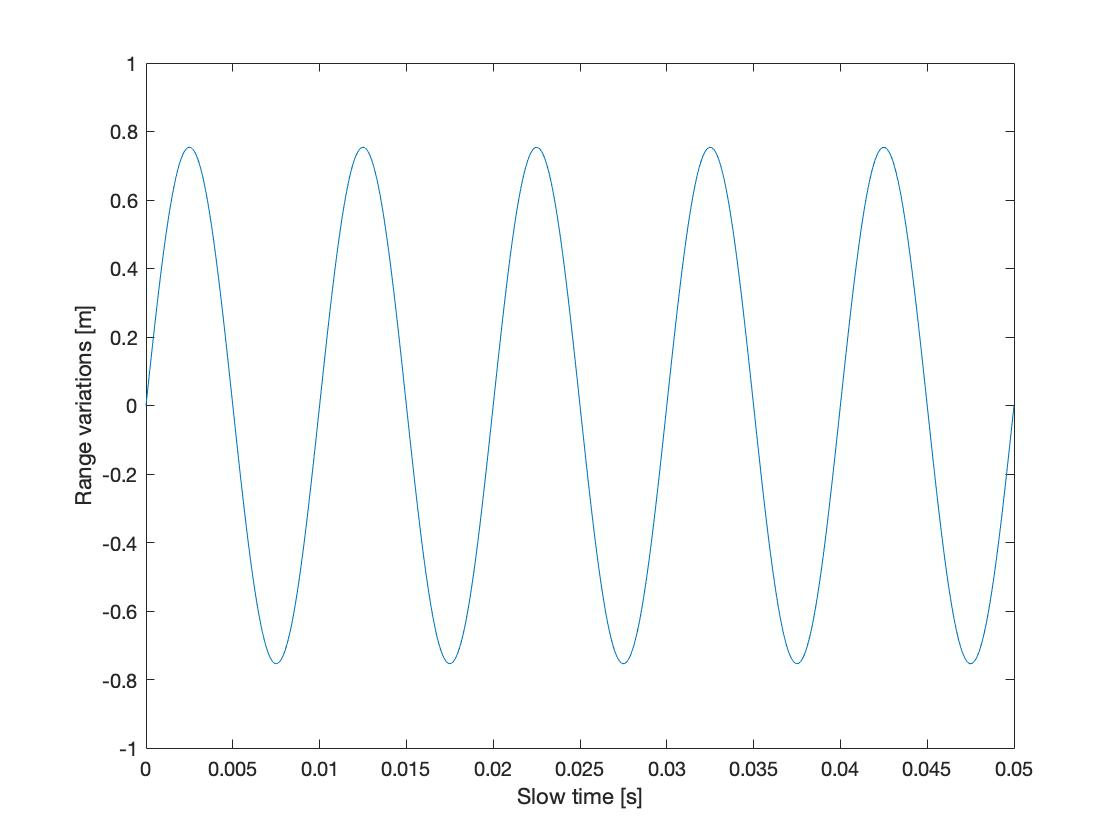
\includegraphics[width=8cm]{Time-frequency analysis-chap3/img/quad_range-slow_time_plot_migration.jpg}
    \caption{Range slow time plot of migrating blade tip of quadcopter drone.}
    \label{range-slow-time-migration-quad}
\end{figure}

In order to avoid this migration the only parameter that can be worked on is the duration of the chirp signal and consequently the slope. Varying the range resolution and thus the bandwidth does not mitigate this problem. In fact, one might intuitively think of increasing the size of the range cells, thus decreasing the bandwidth $B$, to overcome the problem. Unfortunately, the bandwidth is directly proportional to the slope and decreasing it increases the intrapulse Doppler term in the \ref{instafreq}. For example, considering a chirp duration of $T_c = 0.26\;ms$ the migration does not occur as the range change remains within the radar cell. The result of simulation with the new  $T_c$ value can be seen in the figure \ref{no-migration-quad-plot}
\begin{figure}[h!]
    \centering
    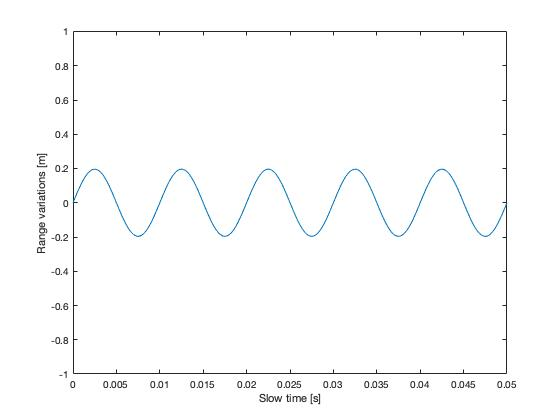
\includegraphics[width=9cm]{Time-frequency analysis-chap3/img/squad_range-slow-time_plot_no_migr.jpg}
    \caption{Range slow time plot of no migrating blade tip of quadcopter drone.}
    \label{no-migration-quad-plot}
\end{figure}

Considering now the case of a drone helicopter whose blades are longer, the range equation model used \ref{rotaionfirstorder} can be simplified. Since in the case of the quadcopter drone whose blade length is on average $\rho = 0.1\;m$, it is entirely contained in a radar cell in the considered case of $\Delta R = 0.2\;m$. In a helicopter drone the blade length is around $\rho = 0.6\;m$, and in this case it occupies $3$ radar cells if the resolution is $\Delta R = 0.2\;m$. So instead of considering the radar range as the distance from the centre of rotation, it is more useful to consider the range as the distance directly from the tip of the blade in order to evaluate only the migration due to the Doppler effect. It is enough in this case to consider null the second term of the \ref{rotaionfirstorder}, that is the projection of the blade tip on the line of sight of the radar. The neglected term in this case is the real migration due to the blade length. $R_0$ is directly the distance between the radar and the tip of the rotating blade. In this case the radar range variations equation becomes: 
\begin{equation}
    R_{var} = R_0 + \frac{c \rho \Omega \sin \left(\Omega t_{s}+\theta_{0}\right)}{\lambda \mu} 
    \label{rangevarhelicopter}
\end{equation} 
The error on the actual distance measurement $R_0$ then becomes:
\begin{equation}
    R_{err} = R_0 - R_{var} = -\frac{c \rho \Omega \sin \left(\Omega t_{s}+\theta_{0}\right)}{\lambda \mu}
\end{equation} 
And its maximum value is therefore:
\begin{equation}
R_{err-max} =  \frac{c \rho \Omega}{\lambda \mu}
\end{equation}
Considering the drone helicopter parameters shown in the \ref{vel_table} table and the radar parameters used so far, the migration is:
\begin{equation}
R_{err-max-helic} = 1.13 m
\end{equation}
That in number of radar cell is:
\begin{equation}
N_{cell-migration} = \frac{R_{err-max-helic}}{\Delta R} \approx 5 
\end{equation}

In the following figure \ref{migrating-helic-drone} the range-slow time plot, result of Matlab simulation with the values of helicpoter drone, is shown. Now the migration is higher due to the longer blade length that determines an higher blade tip velocity.
\begin{figure}[h!]
    \centering
    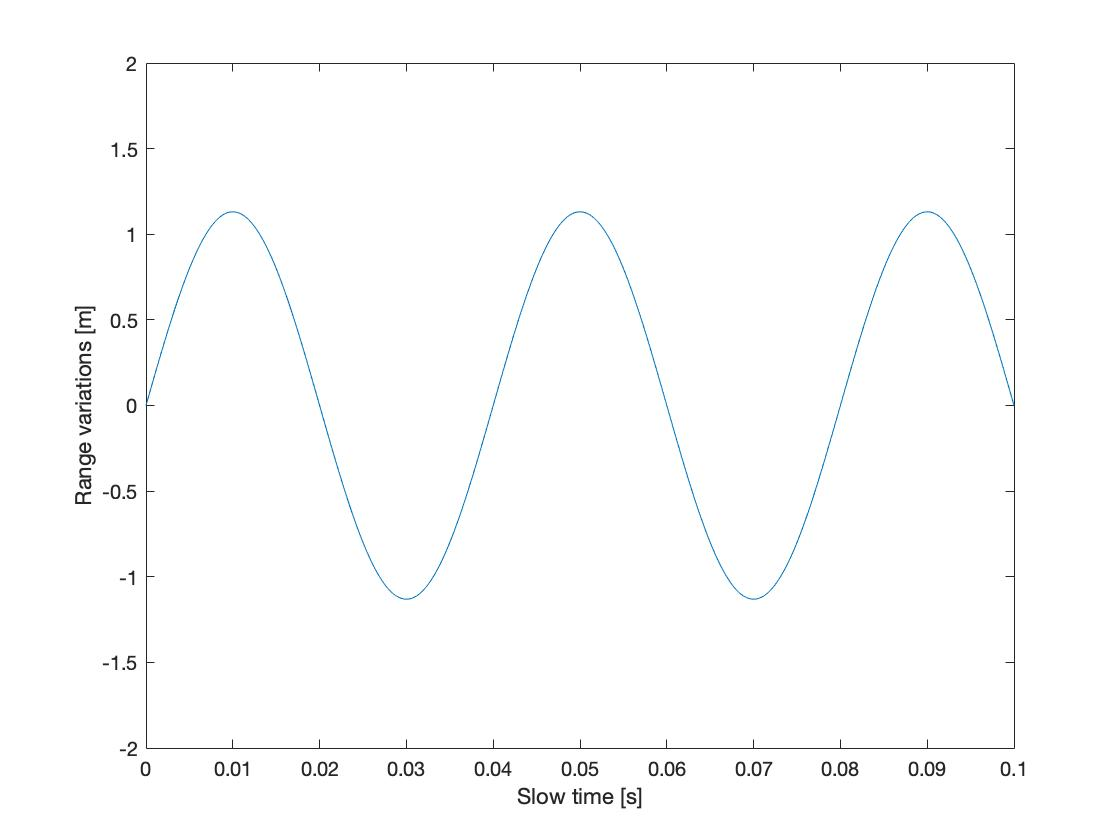
\includegraphics[width=9cm]{Time-frequency analysis-chap3/img/heloc_range_variations_plot.jpg}
    \caption{Range slow time plot of migrating blade tip of helicopter drone.}
    \label{migrating-helic-drone}
\end{figure}
The same argument as above on how to limit this effect still applies. Then decreasing again the duration of the chirp $T_c = 0.17\;ms$ we obtain that the variation remains contained within a radar cell, as shown in the figure \ref{no-migration-helic-plot}.


\begin{figure}[h!]
    \centering
    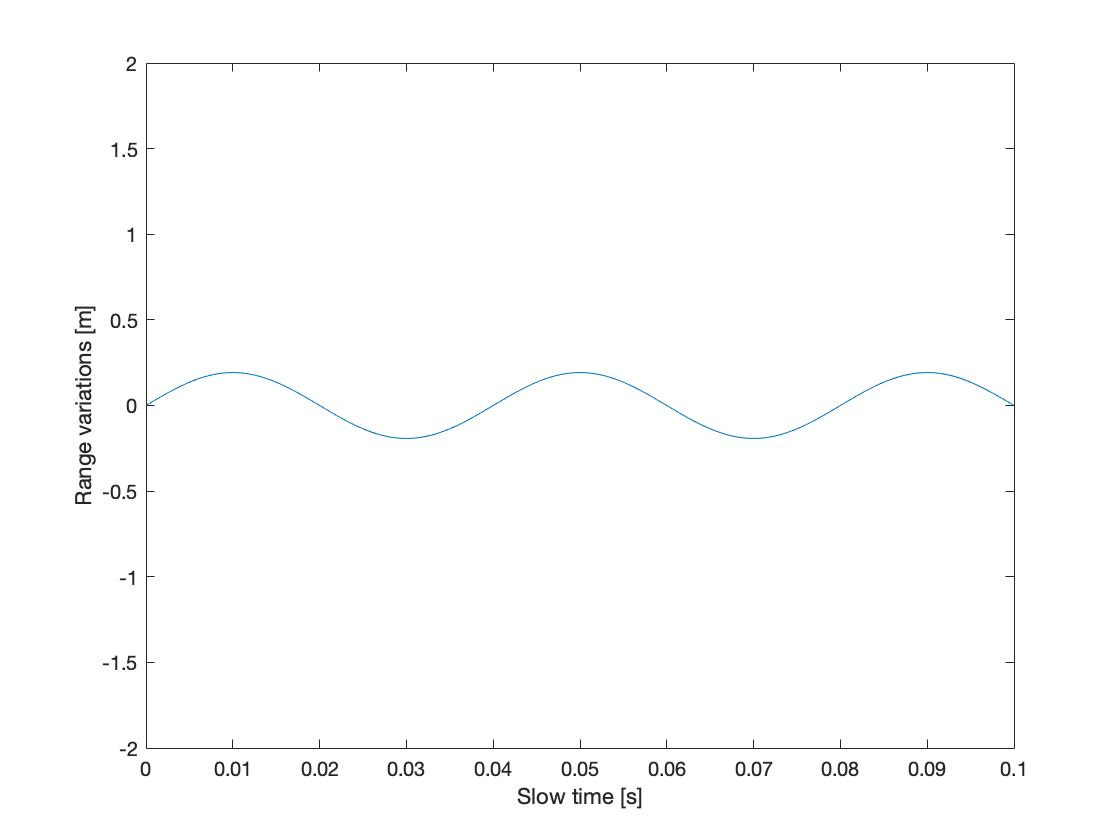
\includegraphics[width=9cm]{Time-frequency analysis-chap3/img/helic_no_range_var_plot.jpg}
    \caption{Range slow time plot of no migrating blade tip of helicopter drone.}
    \label{no-migration-helic-plot}
\end{figure}
Therefore, it is easy to understand that decreasing the duration of the chirp is a way to avoid this bad effect on the process of coherent integration of the pulses received by the target, which prevents to obtain a correct time-frequency analysis. It becomes impossible to correctly visualize all the typical features of a drone spectrogram. An example is shown in the next figure \ref{spect-with-migration}, where the effect of range cell migration due to the rotating blades of a drone occurs in the range-time plane. It thus becomes very simple to observe how the cell variation during the observation time does not allow the extraction of the correct samples containing the spectrogram information. The result is a strange but nevertheless characteristic spectrogram.
\begin{figure}[h!]
    \centering
    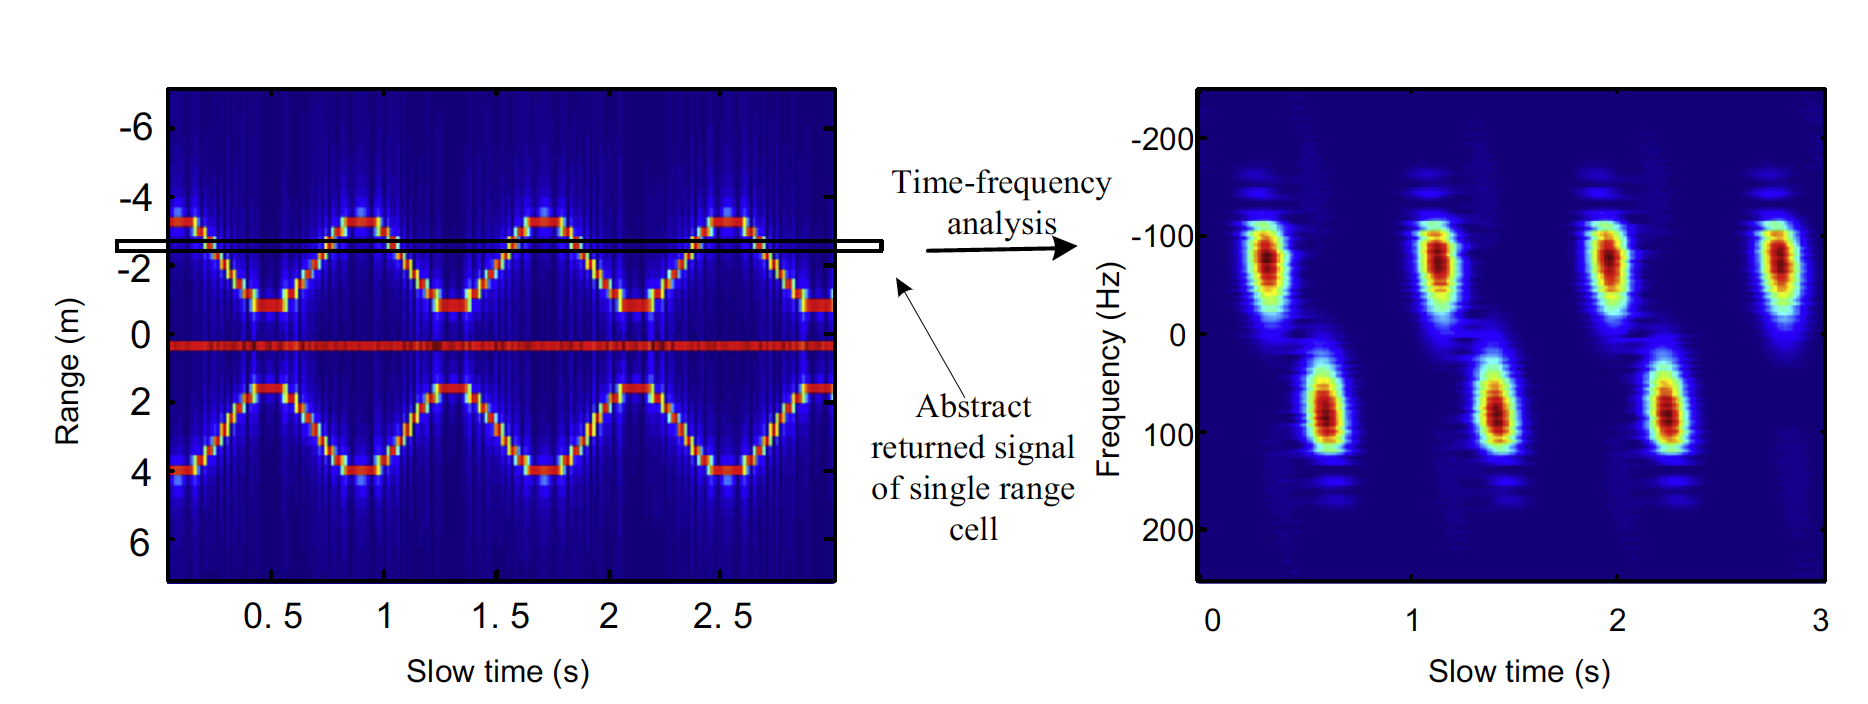
\includegraphics[width=16cm]{Time-frequency analysis-chap3/img/spect with migration.png}
    \caption{Range slow time and time frequency plot of migrating point.\cite{chen_chinese}}
    \label{spect-with-migration}
\end{figure}
The example where the cell migration due to rotation does not occur is in figure \ref{spectr-without-migration}. In this case it is possible to carry out the time-frequency analysis, since the radar cell in which the samples are taken always contains all the necessary information to construct a right spectrogram.
\begin{figure}[h!]
    \centering
    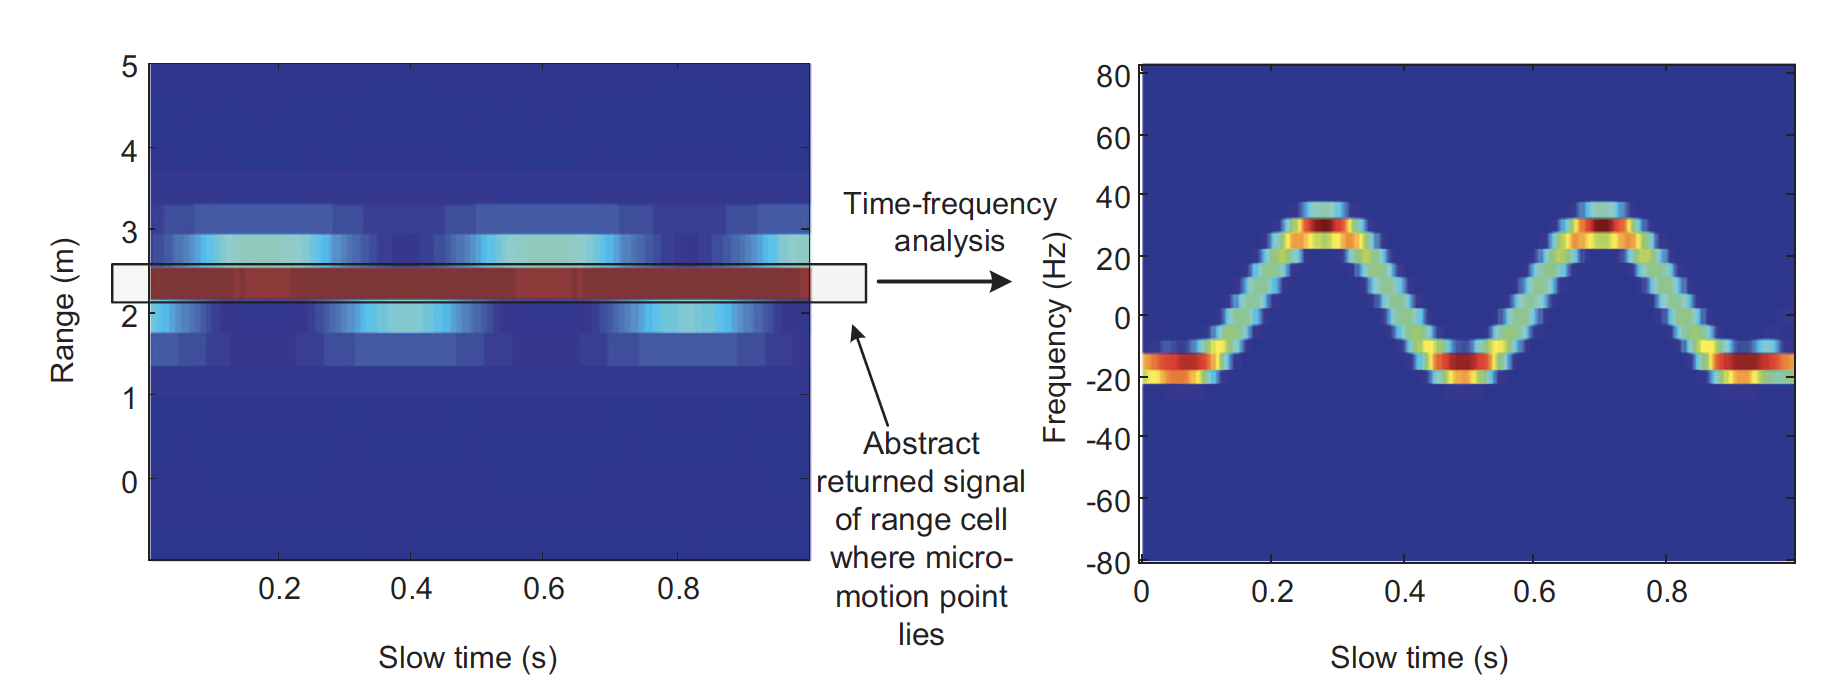
\includegraphics[width=16cm]{Time-frequency analysis-chap3/img/spect without migration.png}
    \caption{Range slow time and time frequency plot of no migrating point.\cite{chen_chinese} }
    \label{spectr-without-migration}
\end{figure}


Referring to the range equation model \ref{rangevarhelicopter} where $R_0$ is the distance to the rotating point, and the last term of the \ref{rangevar} is neglected, mathematically the limit imposed on the duration of the chirp to avoid the occurrence of migration due to rotation is as follows:
\begin{equation}
T_{\text {chirp }}<\frac{\Delta R \lambda B}{\rho \Omega c}
\label{chirp-main-limit}
\end{equation}
It is very important to take \ref{chirp-main-limit} into account during the radar design phase if you want to extract the features of a drone from its spectrogram.

%calcoli caso drone quadcopter ed helicopter e limiti sul parametro Tchirp per evitarlo inserire anche gli esempi grafici del chen sul piano slow time e time frequency di quando si ha rcm e quando no

%descrivo brevemente l'effeto di migrazione che si verifica nello slow time per completezza e anche perchè impone un limite da considerare sul dwell time in fase di design come lo impone la migrazione durante il fast time sul la chirp druration
\subsection{Example of migration in slow time}
Having seen the migration effect that occurs during fast time in the previous section, the same effect that occurs during slow time is now analysed, because the same effect during the slow time impose a constraint on the dwell time. The objective is to highlight the dependency of dwell time and derive the limitations imposed to it in order to avoid every problems during the integration phase. 
The effect of cell migration on a target moving with only radial velocity relative to the radar is shown. The Stop-go model is considered for the received signal.
Starting from the phase of beat signal in function of time (\ref{finalbeat}): 

\begin{equation}
\Phi(t) = \left(-\frac{4 \pi}{c} \mu R t-\frac{4 \pi}{c} f_{c} R+\frac{4 \pi \mu}{c^{2}} R^{2}\right)
\label{phaseofbeat}
\end{equation}

Then applying the range equation in case of Stop-go model approximations:

\begin{equation}
R\left(t_{s}\right)=R_{0}-v_{r} t_{s}
\end{equation}

Applying the definition of time in slow and fast time:

\begin{equation}
    t = t_f + t_s
\end{equation}

The \ref{phaseofbeat} can be rewritten as:

\begin{equation}
\Phi(t_f,t_s) = \left(-\frac{4 \pi}{c} \mu (R_{0}-v_{r} t_{s}) (t_f + t_s)-\frac{4 \pi}{c} f_{c} (R_{0}-v_{r} t_{s})+\frac{4 \pi \mu}{c^{2}} (R_{0}-v_{r} t_{s})^{2}\right)
\end{equation}

Deriving it with respect to $t_s$, dividing for $2\pi$ and neglecting the annoying phase term as discussed in \cite{chen_chinese} we obtain the instant frequency:

\begin{equation}
f=\frac{1}{2 \pi} \frac{\mathrm{d} \Phi(t_s,t_f)}{\mathrm{d} t_s}= -\frac{2 \mu}{c} R_{0}+\frac{2 v_{r}}{\lambda}+\frac{4 \mu}{c} v_{r} t_{s}
\label{insta_freq_beat_slowtime}
\end{equation}

Dividing it by $-2\mu/c$ the range variation is obtained in \ref{rangevarslowtime}. Therefore is not possible discard the third term as in the case of fast time analysis because the value of slow time interval is not so small. For example, transmitting $M = 100$ pulses the slow time interval relative to the last echo received from target is $t_s = 100 T_c$ where $T_c$ as usual is the chirp period.
\begin{equation}
    R_{var}(t_s) = R_0 - \frac{c v_{r}}{\lambda \mu} -2v_r t_s
    \label{rangevarslowtime}
\end{equation} 
The second term of \ref{rangevarslowtime} is constant over time in the case of translating target with constant radial speed, or it's oscillating over time in the case of rotating object. The oscillations due to the rotational motion mainly affect the migration during the fast time, as fully explained in the previous section. In conditions where no migration occurs during the fast time, i.e. the oscillations of the range equation are contained within a radar cell, the possible migration due to the real cell change of the target is now seen.\\
Considering a target moving with radial speed $ v_r = 70km / h $, the FMCW radar with the parameters used up to now, $\Delta R = 0.2\;m$ and $ M = 100 $ signals transmitted to the target each one of $T_{chirp} = 1\;ms$. In these conditions to the 100th echo received, the target will have traveled a space equal to $ v_r 100 T_{chirp} = 1.94\;m$ that is the third term in \ref{rangevarslowtime}, resulting in a migration of:
\begin{equation}
     N_{cell}  = \frac{v_r 100 T_c}{\Delta R} = 9
\end{equation}
In this case a possible solution to this problem is to impose a limit on M and therefore on the observation time.

There are also several techniques that allows to solve the problem without imposing limits on the observation time as explained in \cite{Roos2016RangeMC}.
\begin{equation}
M T_{c} < \frac{\Delta R}{v_r}
\end{equation}
Where $M T_c = t_{dwell}$, then:
\begin{equation}
t_{dwell} < \frac{\Delta R}{v_r}
\end{equation}
As with the limitation on the duration of the chirp signal to avoid migration in the fast time, it is now important to consider this limitation on the dwell time in the design phase to avoid migration during the fast time.


\section{Overview of mD in radar}
A brief summary of the different possibilities of micro Doppler analysis with different radar technologies follows. Before having illustrated  the possible problems such as cell migration, it was easy to think that the micro Doppler analysis only concerned the time-frequency domain. As previously explained, using some wideband radar technologies it is not possible to obtain a correct time frequency analysis and consequently it is not possible to recognize a rotating target in the time-frequency domain. On the other hand, in these cases it is possible to observe the micro Doppler effect on the range-time plane, exploiting the phenomenon of cell migration. So if on the one hand we want to avoid the phenomenon of cell migration to conduct the analysis in the time-frequency domain and recognize a rotating object. On the other hand, we want to exploit the cell migration effect, when it is not possible to avoid it, in order to observe the micro Doppler characteristics in the range-time plane. There are therefore two possible paths depending on the radar technology used. The technology mainly depends on the band, as seen in the previous paragraphs.\\
Radar technologies can be broadly divided into:
\begin{itemize}
    \item Continuous wave radar (CW);
         
    \item Pulse radar;
    
    \item Modulated continuous wave radar (FMCW);
\end{itemize}
In the following subsection each on of these  radar technology is briefly discussed to indicate the possible solutions of micro Doppler analysis that can be conducted.
\subsection{CW radar}
This radar technology is characterized by narrowband signals, in fact the typical signal transmitted by the radar is a sine wave centered on a single frequency, as in \ref{continuouswave}.
\begin{equation}
    s_{tx}(t) = exp(-j2\pi f_0 t)
    \label{continuouswave}
\end{equation}
With this type of radar distance measurements are not possible but it is only possible to measure the speed of the targets by measuring the Doppler frequency and therefore the difference between the transmitted frequency $ f_0 $ and the received echo's frequency.
Therefore, having no information on the range, it is not possible that the cell migration phenomenon  occurs in this case. Using this technology it is theoretically possible to construct a time-frequency analysis and therefore a correct spectrogram of the received signals. Is shown in figure \ref{CWspectrogram} a typical example of a spectrogram constructed using a CW radar. The work in \cite{CWmicroDoppler} shows how it is possible to perform the classification task of different drones, using a continuous wave radar operating at millimeter wave frequencies.
\begin{figure}[h!]
    \centering
    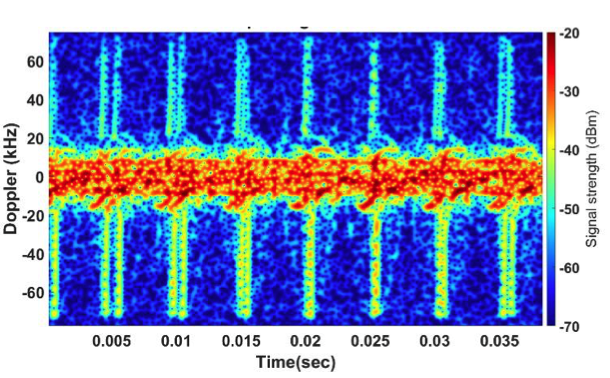
\includegraphics[width=10cm]{Time-frequency analysis-chap3/img/CW micro D spectrogram.png}
    \caption{Spectrogram of quadcopter drone measured with a CW radar.\cite{CWmicroDoppler} }
    \label{CWspectrogram}
\end{figure}
In this case it is therefore possible to use the Stop-go model and all the models of signal received from a drone related to it, as there are no range migration problems. The typical models of received signals from rotor blades that can be used in this case are those presented by V. Chen in \cite{microdoppler_chen}, by Kulpa in \cite{kulpa} and by Martin and Mulgrew in \cite{MartinMulgrew}.


\subsection{Pulse radar}
Pulse radar technology can be subdivided into: 
\begin{itemize}
    \item Simple pulse radar;
    
    \item Compressed pulse radar;
\end{itemize}
The further subdivision is made to break the link between the bandwidth and the temporal duration of the pulse used. This resolves the conflict present in simple pulse radar between resolution in range and resolution in frequency. In fact, the band product per time duration of the pulse $ B \tau $ is 1 in the simple pulse radar. Considering that, to increase the resolution in range a larger bandwidth is required, while to increase the resolution in frequency a greater duration of the pulse is required. Therefore, to achieve a good spatial resolution and at the same time a good frequency resolution, the pulse compression technique is introduced. In practice, a pulse with the desired duration to reach the required frequency resolution level is transmitted, while its frequency is linearly modulated. This is the typical chirp signal described in the previous subsection. So in reception the received echo will be subjected to a cross correlation with the original signal, in the operation described so far as 'dechirp' operation. In this way, all the information related to the phase of the received signal is maintained but at the same time its duration in time is reduced.\\
Returning to the question of time-frequency analysis, with a simple pulse radar it is certainly possible to avoid the phenomenon of cell migration and to continue the micro Doppler analysis in the time-frequency domain without problems. So it's possible to use the Stop-go model and its derivative models to describe received signal from rotor blades.\\
While when a chirped pulse radar is used, it must be checked that during the 'dechirping' operation that take place in the matched filter, there is no range shift due to micro Doppler frequencies. In this case, to verify that the migration does not occur, it is possible to refer to the deviations that occur during the matching operation and assume that they are minimal. As shown in the figure  \ref{Matchingpulsed}.

\begin{figure}[h!]
    \centering
    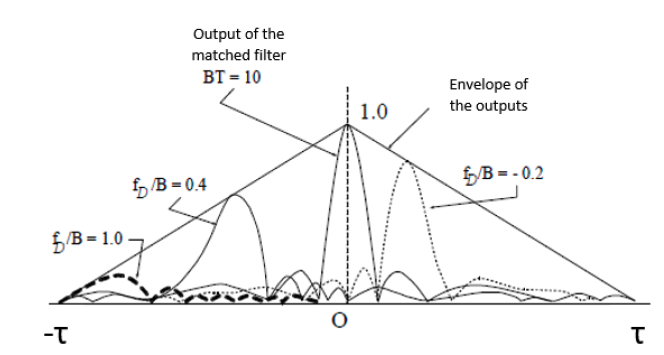
\includegraphics[width=12cm]{Time-frequency analysis-chap3/img/Matching operation.png}
    \caption{Match filtering operation in pulse chirped radar.\cite{galati_radar} }
    \label{Matchingpulsed}
\end{figure}
Assuming in this case that the maximum Doppler frequency in ratio to the signal band is less than a small constant $K$, as showed in \ref{chirpmigrationcond}.

\begin{equation}
\frac{f_{D, \max }}{B} \leq K
\label{chirpmigrationcond}
\end{equation}
If these conditions are met, also in the case of the chirped pulse radar it is possible to use the Stop-go model and its derivatives as the cell migration effect does not occur. In this case it is possible to conduct micro-Doppler analysis in the time-frequency domain.\\
On the contrary, when the relationship \ref{chirpmigrationcond} is not satisfied, it is not possible to carry out the analysis on the time-frequency plane as described in the previous section. In this case it becomes possible to observe the characteristic trend of the range profile of a rotating object as shown in the figure \ref{rangemigrationslowtime}.
\begin{figure}[h!]
    \centering
    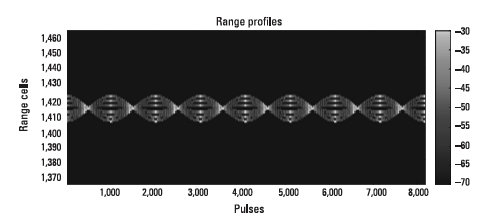
\includegraphics[width=16cm]{Time-frequency analysis-chap3/img/range migration slow time.png}
    \caption{Range slow-time plot of 3 rotor blades .\cite{microdoppler_chen} }
    \label{rangemigrationslowtime}
\end{figure}
In this case the POFACET model is used to decribe the signal returned from each rotor blade, as decribed in \cite{microdoppler_chen}. It is necessary to investigate whether it is possible to extract all the information that is usually extracted from the spectrogram of a rotating object, such as the number of blades, their length, their speed, etc.

\subsection{Modulated continuous wave radar}

In the case of FMCW technology, the band used is much greater than the previous technologies considered. In this condition it becomes much easier to experience the cell migration effect caused by a rotating object. Whether or not the effect occurs depends mainly on the available band, as it increases, as well the resolution in range increases and it becomes simpler that the migration of a rotating object occurs. This is the technology most prone to the migration effect. At the same time, however, it is possible to avoid the migration phenomenon by appropriately choosing the radar parameters and in particular the duration of the ramps $T_{chirp}$, as shown in the previous section. Recalling, the relationship that must be met to avoid migration is the \ref{chirp-main-limit}:
\begin{equation}
T_{\text {chirp }}<\frac{\Delta R \lambda B}{\rho \Omega c}
\end{equation}
Where:
\begin{itemize}
    \item $\Delta R$ is the range resolution;
    
    \item \textbf{$\lambda$} is the wavelength;
    \item \textbf{$B$} is the bandwidth;
    \item \textbf{$\rho$} is the amplitude of rotation;
    \item \textbf{$\Omega$} is the rotation rate;
    \item \textbf{$c$} is the light speed;
\end{itemize}
If this condition is satisfied it is possible to carry out the analysis on the time-frequency plane. It depends on the specific case considered, for example in the case considered with the FMCW radar parameters of the previous section, the migration effect could be avoided with a chirp duration equal at most to $T_{chirp} = 0.17\;ms $. The case considered is of an helicopter drone which is more affected by the migration phenomenon due to the higher radial speed of the blade tip. While for a quadcopter drone a duration at most of $T_{chirp} = 0.26\;ms $ is sufficient, as the radial speed of the blade tip is lower.\\
On the other hand, this limit could result in a ramp duration that is not physically possible or in any case can produce a value of $T_{chirp}$ too expensive to implement in the real world. In cases where it is not possible to satisfy the \ref{chirp-main-limit} it is therefore necessary to move the micro-Doppler analysis on the range-time plane to highlight the migration phenomenon of the cell and extract the information on the rotating object from it as it is possible to observe in figure \ref{rangemigrationslowtime}.
\subsection{Summary}
From what has been said in the previous chapters, it is possible to carry out micro-Doppler analysis on both the Range-Time and Frequency-Time planes, depending on whether the Range Migration effect occurs or not. 
Among all the above radar solutions, there are two possible ways to perform micro-Doppler analysis at low cost, i.e. limiting the cost of the radar components and the final cost as a whole.
Consequently, in order to achieve the goal of obtaining a low cost radar capable of performing this analysis there are two possibilities.
\begin{itemize}
    \item CW radar solution: it is possible to carry out micro-Doppler analysis by means of a continuous wave radar, making an important sacrifice on the data measured by the radar, in particular by accepting not to measure the distance at which the drone is located, but simply to carry out identification tasks by means of time-frequency analysis. By using this type of radar, it is ensured that there is no migration effect, and consequently it is possible to conduct the analysis on the time-frequency plane without any problems and keeping the cost of the radar low.;
    
    \item FMCW radar solution: Using a linear frequency modulation radar also makes it possible to measure the distance at which the drone is located. It is therefore possible to carry out detection tasks and not only identification tasks as with CW radar. Furthermore, by using this radar, we have the benefit of being able to carry out the identification task by means of micro-Doppler analysis both in the time-frequency plane and in the range-time plane. In this case we have a hybrid solution, in which by modifying the duration of the waveform we can decide on which of the two planes we want to conduct the analysis. In the end, depending on the situation and the costs of the radar components, it is possible to choose which of the two analyses is the most economical.


\end{itemize}
The second way, i.e. using a radar FMCW, leaves far more opportunities open than using a simple radar CW. A much more complete result could be obtained for the almost same cost. In addition, the biggest benefit is in the number of analysis paths that remain open when choosing an FMCW radar solution. Unlike the CW radar case, which precludes the possibility of performing micro-Doppler analysis in the range-time plane, the FMCW radar leaves open two roads that can be taken depending on the chirp used. One could even think of implementing a hybrid solution, in which the duration of the waveform is varied as needed and therefore one analysis is preferred over the other.\\
The objective of the next chapter is to analyse the FMCW radar parameters and their limits, with the aim first of carrying out analyses on the Range-time plane and then on the Freqeuncy-time plane. At the end, after having described and carried out the design of the radar and its waveform for the two cases, it is possible to choose the one which optimises the costs and the results obtained. 
